\chapter{行动和状态}
\label{chap:dynamical-systems-and-state-estimation}
\label{chap:action-and-state}

给房间施加同样的加热量，下一时刻的温度仍取决于房间现在有多热。只记录当前
输入，不能预测未来；逐项保存全部加热历史，又未必必要。状态模型在两者之间作出
选择：用一个当前量保存历史对未来仍有用的作用，再规定这个量怎样更新。
第~\ref{chap:signal-analysis}章研究输入与输出之间的信号映射，本章打开映射内部，
研究状态怎样承接过去、怎样受行动推动，以及传感器不直接显示状态时怎样推断它。

本章把行动当作给定输入，不选择行动策略。贯穿例中的状态$x_t$是相对于环境温度的
温差，输入$u_t$是加热量，无噪声时满足$x_{t+1}=0.8x_t+u_t$。
给定初值与输入以后，我们先求轨迹，继而判断扰动是否消退；加入过程噪声，
求解对象变为随机轨迹及其分布；再加入传感器读数，才形成观测条件下的状态分布。
一条轨迹、一个时刻的边缘分布、多个时刻的联合分布和观测后的后验分布分别回答
不同问题。数值方法也须说明它在近似其中哪一个对象。

\section{行动与状态的演化模型}
\label{sec:dynamical-difference-ode}

\subsection{状态、输入与初始条件}

状态是模型认为足以接续未来演化的当前信息，不必是全部可见数据，也不必逐项保存
历史。以温度为例，在固定环境与采样间隔下，取状态空间为$\mathbb R$，给定初值
$x_0=0$，并持续施加$u_t=0.4$，则最初几步为
\[
  x_1=0.4,\qquad x_2=0.72,\qquad x_3=0.976.
\]
这里的系数$0.8$表示前一时刻温差保留下来的比例；其余影响由输入补充。
恒定状态$r=2$所需的输入恰为$r-0.8r=0.4$。这只是给定输入下的平衡核对，
并未根据当前温度改变行动。

状态的选择依赖模型。若墙体蓄热显著影响下一步室温，而当前室温无法概括它，
就要增加墙体温度等状态；若传感器有滞后，还应区分房间状态与传感器内部状态。
所谓“当前状态足够”，是一项需要验证的建模要求，不是把某个变量命名为状态后
自动获得的性质。

初始条件规定轨迹从哪里开始，输入规定沿途施加什么作用，演化规律规定这些作用
怎样改变状态。输出则是模型对外显示的量。无噪声且传感器直接测温时可以有
$y_t=x_t$，但一般输出只给状态的部分信息。后文恢复过程噪声与观测噪声时，
仍使用同一时序：时刻$t$的状态已经形成，传感器产生$y_t$，然后给定的$u_t$
把状态推向$t+1$。只有在控制问题中，才进一步规定如何依据这些信息选择$u_t$。

\subsection{离散时间的状态更新}

设$\mathcal X$是允许的状态集合，$\mathcal U$是输入集合。一步更新映射
\[
  F_t:\mathcal X\times\mathcal U\longrightarrow\mathcal X,\qquad
  \bm x_{t+1}=F_t(\bm x_t,\bm u_t)
\]
直接规定下一状态。只要初值属于$\mathcal X$、每个输入属于$\mathcal U$，且映射
确实把状态送回$\mathcal X$，有限步递推便有定义。若只在某个区域内给出公式，
则每一步还要检查结果是否留在该区域。本文温度例暂不加输入或状态约束。

线性模型常写为
\[
  \bm x_{t+1}=\bm A_t\bm x_t+\bm B_t\bm u_t,\qquad
  \bm x_t\in\mathbb R^d,\quad \bm u_t\in\mathbb R^m.
\]
它关于状态与输入的联合变量是线性的；固定非零输入后，它关于状态通常是仿射的。
矩阵不随$t$改变称为时不变，显式随$t$改变则称为时变。是否线性与是否时变是两项
独立性质。若$\bm A_t$还依赖当前状态或输入，虽然公式仍有“矩阵乘状态”的外形，
整体映射通常已不是线性的。

一个可直接计算的模型是带泄漏的记忆：
\begin{equation}
  x_{t+1}=a x_t+b u_t,\qquad x_0\ \text{给定}.
  \label{eq:dynamical-leaky-discrete-memory}
\end{equation}
温度例对应$a=0.8,b=1$。系数$a$控制已有信息保留多少，$b$控制新输入进入多少。
能逐步计算并不说明长期状态有界；同一公式取$|a|>1$便可能放大早期扰动。

\subsection{连续时间的状态变化}

若关注相邻采样时刻之间发生了什么，需要规定瞬时变化率，而不仅是相隔一步的差值。
常微分方程（ordinary differential equation, ODE）初值问题写为
\begin{equation}
  \dot{\bm x}(t)=\bm f(t,\bm x(t),\bm u(t)),\qquad
  \bm x(t_0)=\bm x_0.
  \label{eq:dynamical-general-ivp}
\end{equation}
给定输入后，右侧是作用在当前状态上的向量场。若它不显含时间，称方程为自治的；
否则为非自治的。恒定矩阵配上随时间变化的外部输入，也会产生非自治方程。
向量场告诉我们“现在往哪里、以多快速度移动”，有限时间转移还要由积分确定。

例如把泄漏记忆在小间隔$\Delta t$上的系数写为
$a=1-\lambda\Delta t$、$b=\Delta t$，形式上有
\[
  \frac{x_{t+\Delta t}-x_t}{\Delta t}=-\lambda x_t+u_t.
\]
若极限成立，对应模型为
\begin{equation}
  \dot x(t)=-\lambda x(t)+u(t).
  \label{eq:dynamical-leaky-continuous-memory}
\end{equation}
这说明连续变化率怎样导出一种离散近似，而不是说明任意离散系数都与某个连续模型
天然等价。特别是贯穿例的$0.8$是已给定的一步系数，不在此悄然换成另一种采样约定。

并非所有系统都耗散已有状态。位置相同但速度不同的运动会有不同未来，因此力学中
常把位置和动量合在一起作为状态；这个状态所在的空间称为相空间。
\begin{definition}[可分Hamilton系统]
  \label{def:dynamical-separable-hamiltonian-system}
  令$\bm q,\bm p\in\mathbb R^d$分别为位置与动量，$U$为连续可微的势能，
  $\bm M$为对称正定的质量矩阵。可分Hamilton量为
  \begin{equation}
    H(\bm q,\bm p)=U(\bm q)+\frac12\bm p^\top\bm M^{-1}\bm p.
    \label{eq:dynamical-separable-hamiltonian}
  \end{equation}
  相应的Hamilton方程为
  \begin{equation}
    \dot{\bm q}=\nabla_{\bm p}H,\qquad
    \dot{\bm p}=-\nabla_{\bm q}H.
    \label{eq:dynamical-hamilton-equations}
  \end{equation}
\end{definition}
第一式由动量得到位置速度，第二式由势能坡度得到动量变化。令
$\bm z=(\bm q^\top,\bm p^\top)^\top$，则方程也可写为
\[
  \dot{\bm z}=\bm J\nabla H(\bm z),\qquad
  \bm J=\begin{bmatrix}\bm0&\bm I\\-\bm I&\bm0\end{bmatrix}.
\]
它不是沿$-\nabla H$下降，而是把梯度转换为成对坐标之间的运动方向。
例如$U(q)=q^2/2,M=1$给出$\dot q=p,\dot p=-q$，位置与动量轮流交换。
轨迹是否唯一、能量是否保持、怎样数值推进，将分别在相应条件下证明。

\section{状态轨迹的求解与计算}
\label{sec:action-state-trajectory-computation}

模型给出局部规则，轨迹则把这些规则接续起来。离散时间可以有限次复合；连续时间
需要先证明积分方程有解。轨迹确定以后，才能讨论历史输入的贡献、保守运动的几何
以及计算误差。以下各项都固定初值与输入，不把未知观测混入求解条件。

\subsection{给定初值与输入的轨迹求解}

\subsubsection{离散时间下的轨迹递推}

把给定输入吸收进$F_t^{\bm u}(\bm x)=F_t(\bm x,\bm u_t)$，前两步为
\[
  \bm x_1=F_0^{\bm u}(\bm x_0),\qquad
  \bm x_2=F_1^{\bm u}\bigl(F_0^{\bm u}(\bm x_0)\bigr).
\]
一般状态是有序复合
$\bm x_t=(F_{t-1}^{\bm u}\circ\cdots\circ F_0^{\bm u})(\bm x_0)$。
较晚更新写在左边，因为它作用于较早更新的结果；调换复合顺序会改变系统。

泄漏模型可进一步展开：
\begin{equation}
  x_t=a^t x_0+\sum_{j=0}^{t-1}a^{t-1-j}b u_j.
  \label{eq:dynamical-discrete-variation-constants}
\end{equation}
证明从$t=0$的空和开始。若式子对$t$成立，两边乘$a$再加$b u_t$，
便得到$t+1$的式子。初值与每次输入的贡献都在其中：旧输入经历的更新次数更多，
因而多乘若干个$a$。

取独立于温度任务的泄漏例$a=1/2,b=1,x_0=0$。仅在第零步输入$u_0=1$时，
$x_1=1,x_2=1/2,x_3=1/4$；若$u_0=u_1=1$，则$x_2=3/2$，
其中$1/2$来自旧输入，$1$来自新输入。这就是状态保存的历史总作用。
回到温度例，$u_t=0.4$给出
\[
  x_t=2+0.8^t(x_0-2).
\]
有限步展开已经得到轨迹；它趋于$2$还使用了$|0.8|<1$。一般非线性映射可逐步计算，
却未必有这样的闭式或极限。

\subsubsection{连续时间下的轨迹存在与延拓}

一个“几乎处处给出斜率”的公式，要能恢复整条曲线，必须排除没有被导数记录的
奇异变化。为此采用绝对连续曲线，而非任意连续曲线。
\begin{definition}[绝对连续曲线]
  \label{def:dynamical-absolutely-continuous-curve}
  有限区间$[a,b]$上的曲线$\bm x:[a,b]\to\mathbb R^d$称为
  \term{绝对连续曲线}，若存在$\bm v\in L^1([a,b];\mathbb R^d)$，使
  $\bm x(t)=\bm x(a)+\int_a^t\bm v(s)\,\mathrm ds$对每个$t$成立。
  此时$\dot{\bm x}=\bm v$几乎处处成立。
\end{definition}
记$\bm g(t,\bm x)=\bm f(t,\bm x,\bm u(t))$。积分意义下的解就是满足
\begin{equation}
  \bm x(t)=\bm x_0+\int_{t_0}^t\bm g(s,\bm x(s))\,\mathrm ds
  \label{eq:dynamical-ivp-integral-form}
\end{equation}
的绝对连续曲线。当$\bm g$连续时，它还是处处满足微分方程的经典解。

\begin{theorem}[局部存在唯一性]
  \label{thm:dynamical-picard-lindelof}
  若给定输入后的$\bm g$在$(t_0,\bm x_0)$附近连续，且关于状态局部Lipschitz，
  Lipschitz常数可在该时间邻域内统一选取，则存在包含$t_0$的区间，使
  式~\eqref{eq:dynamical-general-ivp}有唯一局部解。
\end{theorem}
\begin{proof}
  在适用邻域内选闭区域
  \[
    D=[t_0-a,t_0+a]\times
    \{\bm x:\|\bm x-\bm x_0\|_2\leq b\}.
  \]
  紧性给出$M=\sup_D\|\bm g\|_2<\infty$；记统一Lipschitz常数为$L$。
  选$h>0$使$h\leq a,Mh\leq b,Lh<1$。在$I=[t_0-h,t_0+h]$上，
  \[
    \mathcal X=\{\bm z\in C(I,\mathbb R^d):
       \|\bm z-\bm x_0\|_\infty\leq b\}
  \]
  是完备空间的闭子集，因而完备。定义
  $(\mathcal T\bm z)(t)=\bm x_0+\int_{t_0}^t\bm g(s,\bm z(s))\,\mathrm ds$。
  对$\bm z\in\mathcal X$，
  $\|(\mathcal T\bm z)(t)-\bm x_0\|_2\leq M|t-t_0|\leq Mh\leq b$，
  所以$\mathcal T$映回$\mathcal X$。同时
  \[
    \|\mathcal T\bm z_1-\mathcal T\bm z_2\|_\infty
    \leq Lh\|\bm z_1-\bm z_2\|_\infty.
  \]
  压缩映射定理给出唯一不动点，即积分方程的解。任何同初值的局部解在足够短的
  区间内都落在$\mathcal X$，故与此解重合；在共同存在区间逐段重复便得到局部唯一性。
\end{proof}

这个证明把三种条件分开使用：连续性给出有界的局部变化率，完备性让迭代的极限仍是
候选曲线，统一Lipschitz条件使积分算子在短区间收缩。只有连续性不保证唯一性。
例如$\dot x=\sqrt{|x|},x(0)=0$既有零解，也有对任意$c\geq0$定义的
\[
  x(t)=
  \begin{cases}
    0,&0\leq t\leq c,\\
    (t-c)^2/4,&t>c.
  \end{cases}
\]
解可以任意等待后再离开原点。

局部解能通过重叠区间的唯一性接成长一些的解。不能再向外接续的解称为最大解；
最大区间包含全部所需时刻时，才得到相应的全局解。局部光滑仍可能有限时间爆炸：
$\dot x=x^2,x(0)=1$的解$x(t)=1/(1-t)$在$t=1$前已无界。
排除这种情况，需要增长控制。下面的估计也是后文比较两条轨迹的共同工具。

\begin{lemma}[Grönwall积分估计]
  \label{lem:action-state-gronwall}
  设$e$为$[a,T]$上非负连续函数，$b$为非负可积函数。若
  \[
    e(t)\leq c+\int_a^t b(s)e(s)\,\mathrm ds,\qquad c\geq0,
  \]
  则$e(t)\leq c\exp(\int_a^t b(s)\,\mathrm ds)$。
  更一般地，若右侧另有$\int_a^t r(s)\,\mathrm ds$，其中$r\geq0$可积，则
  \[
    e(t)\leq c\,\mathrm e^{\int_a^t b}
      +\int_a^t r(s)\,\mathrm e^{\int_s^t b}\,\mathrm ds.
  \]
\end{lemma}
\begin{proof}
  令$E(t)=c+\int_a^t[b(s)e(s)+r(s)]\,\mathrm ds$，则$e\leq E$，
  且$E'\leq bE+r$几乎处处成立。乘以绝对连续的积分因子
  $\exp(-\int_a^t b)$，使用乘积法则并从$a$积分到$t$，得
  \[
    E(t)\mathrm e^{-\int_a^t b}
    \leq c+\int_a^t r(s)\mathrm e^{-\int_a^s b}\,\mathrm ds.
  \]
  再乘回积分因子并用$e\leq E$即可；取$r=0$得到第一式。
\end{proof}

若$\|\bm g(t,\bm x)\|\leq b(t)\|\bm x\|+r(t)$，其中$b,r$在每个有限时间区间
可积，积分方程与此引理给出有限的状态上界。在局部存在条件持续有效、状态域为
$\mathbb R^d$时，这排除了有限时间逃逸，因而最大解可延拓到任意有限时刻。
全局Lipschitz以及$\|\bm g(t,\bm0)\|$的局部可积性是常用的充分条件。
对仅时间可测的输入还需相应的Carathéodory条件：$\bm g$关于时间可测、
关于状态连续，并在紧状态集上有可积上界与可积Lipschitz系数。不能把上述连续
输入版本的局部定理原样套给任意不可测输入。

\subsection{历史输入的传播与表示}

一个已经给定的状态递推怎样传播旧输入，与怎样设计状态来近似一段历史，是两个
方向相反的问题。前者展开已有方程，后者选择要保存的坐标。线性传播和投影分别使
这两个问题可计算。

\subsubsection{线性状态下的历史输入传播}
\label{sec:signal-analysis-state-history-kernels}

先保持离散时间。对时不变系统，允许输出还直接依赖当前输入：
\begin{align}
  \bm x_{t+1}&=\bm A\bm x_t+\bm B\bm u_t,\notag\\
  \bm y_t&=\bm C\bm x_t+\bm D\bm u_t.
  \label{eq:signal-analysis-lti-state-space}
\end{align}
这里$\bm A\in\mathbb R^{d\times d}$、$\bm B\in\mathbb R^{d\times m}$、
$\bm C\in\mathbb R^{p\times d}$、$\bm D\in\mathbb R^{p\times m}$。
本章统一用$\bm x$表示状态、$\bm u$表示输入；信号表示中的输入记号不能在这里
继续兼作状态。直接项$\bm D\bm u_t$是本小节允许的一般输出通道，贯穿温度
传感器模型则取$\bm D=\bm0$，不改变“先读数、后输入推动下一状态”的时序。

前两步为$\bm x_1=\bm A\bm x_0+\bm B\bm u_0$及
$\bm x_2=\bm A^2\bm x_0+\bm A\bm B\bm u_0+\bm B\bm u_1$。归纳得到
\begin{equation}
  \bm x_t=\bm A^t\bm x_0+
    \sum_{\tau=0}^{t-1}\bm A^{t-1-\tau}\bm B\bm u_\tau.
  \label{eq:signal-analysis-state-unrolling}
\end{equation}
归纳步把右侧乘$\bm A$并加$\bm B\bm u_t$，求和上界与各项幂次就同时前移一格。
代入输出方程，
\begin{equation}
  \bm y_t=\bm C\bm A^t\bm x_0+\bm D\bm u_t+
    \sum_{\tau=0}^{t-1}\bm C\bm A^{t-1-\tau}\bm B\bm u_\tau.
  \label{eq:signal-analysis-state-convolution}
\end{equation}
第一项是初态的自由响应，其余项是输入响应。零初态时，定义
\begin{equation}
  \bm K_0=\bm D,\qquad
  \bm K_r=\bm C\bm A^{r-1}\bm B\quad(r\geq1),
  \label{eq:signal-analysis-state-kernel}
\end{equation}
就得到因果卷积$\bm y_t=\sum_{\tau=0}^t\bm K_{t-\tau}\bm u_\tau$。
核$\bm K_r$记录$r$步以前的输入经过剩余状态传播后对当前输出的作用。
非零初态的自由响应必须另加，不能塞进一个与输入无关的零状态卷积公式。

用标量$a=1/2,b=c=1,d=0,x_0=0$核对。依次输入
$u_0=1,u_1=2,u_2=1$，递推给出
$y_0=0,y_1=1,y_2=5/2,y_3=9/4$。核为
$K_0=0,K_1=1,K_2=1/2,K_3=1/4$，所以
\[
  y_3=K_3u_0+K_2u_1+K_1u_2=\frac14+1+1=\frac94.
\]
严格因果的状态通道使$y_0=0$；若$d\neq0$，当前输入还会立即通过$K_0=d$进入
输出。标量核$ca^{r-1}b$在$|a|<1$时几何衰减，在$|a|>1$时增长；多维状态
还需检查不同方向的传播，不能由核的形式本身断言稳定。

时变系统用有序乘积
\[
  \bm\Phi(t,s)=\bm A_{t-1}\cdots\bm A_s\quad(t>s),\qquad
  \bm\Phi(s,s)=\bm I
\]
传播齐次状态，于是
\[
  \bm x_t=\bm\Phi(t,0)\bm x_0+
    \sum_{\tau=0}^{t-1}\bm\Phi(t,\tau+1)\bm B_\tau\bm u_\tau.
\]
若输出为$\bm C_t\bm x_t+\bm D_t\bm u_t$，对应核为
\[
  \bm K_{t,t}=\bm D_t,\qquad
  \bm K_{t,\tau}=\bm C_t\bm\Phi(t,\tau+1)\bm B_\tau\quad(\tau<t).
\]
它依赖两个绝对时刻，通常不只依赖滞后$t-\tau$，所以线性仍在，平移不变性却已
消失。较晚矩阵必须置于左边。若这些矩阵还依赖输入或状态，展开系数也随输入轨迹
改变，叠加通常失效；固定轨迹附近的线性化核仅有局部含义。

连续时间对应的时不变方程是
\begin{equation}
  \dot{\bm x}(t)=\bm A\bm x(t)+\bm B\bm u(t).
  \label{eq:dynamical-lti-continuous}
\end{equation}
矩阵指数的导数见第~\ref{chap:matrix-analysis}章。令
$\bm z(t)=\mathrm e^{-t\bm A}\bm x(t)$，乘积求导给出
$\dot{\bm z}(t)=\mathrm e^{-t\bm A}\bm B\bm u(t)$。积分并乘回指数，得到
\begin{equation}
  \bm x(t)=\mathrm e^{(t-t_0)\bm A}\bm x_0+
    \int_{t_0}^t\mathrm e^{(t-s)\bm A}\bm B\bm u(s)\,\mathrm ds.
  \label{eq:dynamical-lti-variation-constants}
\end{equation}
代入$t_0$得到初值；对积分上限求导得到原方程，因而这确实是解，而非只是一种
形式展开。局部可积输入给出积分意义的解，连续输入给出经典解。标量泄漏模型取
$\lambda>0,u(t)\equiv u_0$时，
\[
  x(t)=\mathrm e^{-\lambda(t-t_0)}x_0+
    \frac{1-\mathrm e^{-\lambda(t-t_0)}}{\lambda}u_0.
\]
初值作用消退，持续输入则留下$u_0/\lambda$，两种贡献不能一起称为“趋零”。

时变系数需要连续时间的传播算子。
\begin{definition}[状态转移矩阵]
  \label{def:dynamical-state-transition-matrix}
  对连续矩阵函数$\bm A(t)$，\term{状态转移矩阵}$\bm\Phi(t,s)$是满足
  \begin{equation}
    \partial_t\bm\Phi(t,s)=\bm A(t)\bm\Phi(t,s),\qquad
    \bm\Phi(s,s)=\bm I
    \label{eq:dynamical-state-transition-matrix}
  \end{equation}
  的矩阵值解。它把时刻$s$的齐次初态映到时刻$t$。
\end{definition}
由解的唯一性，$\bm\Phi(t,r)\bm\Phi(r,s)=\bm\Phi(t,s)$。
反向传播给出$\bm\Phi(t,s)^{-1}=\bm\Phi(s,t)$；用该逆矩阵作积分因子，得到
\begin{equation}
  \bm x(t)=\bm\Phi(t,t_0)\bm x_0+
    \int_{t_0}^t\bm\Phi(t,s)\bm B(s)\bm u(s)\,\mathrm ds.
  \label{eq:dynamical-ltv-variation-constants}
\end{equation}
对输出$\bm C(t)\bm x(t)+\bm D(t)\bm u(t)$，连续历史核是
$\bm C(t)\bm\Phi(t,s)\bm B(s)$，直接项仍单列。时不变时它退化为滞后核
$\bm C\mathrm e^{(t-s)\bm A}\bm B$。

一般不能令$\bm\Phi(t,s)=\exp(\int_s^t\bm A(r)\,\mathrm dr)$。
例如先运行常矩阵$\bm A_1$一单位时间，再运行$\bm A_2$一单位时间，实际传播为
$\mathrm e^{\bm A_2}\mathrm e^{\bm A_1}$，非交换时不等于
$\mathrm e^{\bm A_1+\bm A_2}$。只有不同时间矩阵彼此交换等附加条件成立时，
才能把时序传播压成普通矩阵指数。

\subsubsection{有限维状态下的历史窗口表示}

另一种构造从希望保留的历史特征出发。例如为一段输入保留平均值与线性趋势，
就可把投影坐标当作状态。设随$t$改变的内积为
\[
  \langle f,g\rangle_t=\int_0^t f(s)g(s)w_t(s)\,\mathrm ds,
\]
并选基$\phi_1^{(t)},\ldots,\phi_d^{(t)}$。若基正交归一，
$c_i(t)=\langle u,\phi_i^{(t)}\rangle_t$就是展开系数；一般基则要先构造
$G_{i,j}(t)=\langle\phi_i^{(t)},\phi_j^{(t)}\rangle_t$，
再由$\bm G(t)\bm a(t)=\bm c(t)$得到投影坐标$\bm a(t)$。
分析坐标$\bm c$和投影坐标$\bm a$不能在非正交基下混用。

窗口本身移动时，状态变化不全来自新输入。固定宽度$T>0$，写
\[
  c_\ell(t)=\int_{t-T}^t u(s)\phi_\ell(t,s)w(t,s)\,\mathrm ds.
\]
在被积函数及所需偏导连续等Leibniz求导条件下，
\begin{align}
  \dot c_\ell(t)
  ={}&u(t)\phi_\ell(t,t)w(t,t)
    -u(t-T)\phi_\ell(t,t-T)w(t,t-T)\notag\\
  &+\int_{t-T}^t u(s)\partial_t[\phi_\ell(t,s)w(t,s)]\,\mathrm ds.
  \label{eq:dynamical-moving-window-coefficient}
\end{align}
这三项分别来自右端新输入、左端旧输入退出，以及窗口内部基或权重的改变。
漏掉左端项，就把固定长度窗口误当成只增长不遗忘的历史。

取均匀权重下的常数与一次矩，
\[
  c_0(t)=\frac1T\int_{t-T}^t u(s)\,\mathrm ds,\qquad
  c_1(t)=\frac2{T^2}\int_{t-T}^t(s-t+T)u(s)\,\mathrm ds,
\]
上式给出
\[
  \dot c_0(t)=\frac{u(t)-u(t-T)}T,\qquad
  \dot c_1(t)=\frac2T u(t)-\frac2T c_0(t).
\]
第二式在当前坐标与当前输入之间闭合，第一式仍需要窗口左端的值。
所以有限个历史特征不自动形成能独立接续演化的有限维状态；需要额外状态、特别的
基与权重，或对边界项作近似。

HiPPO一类方法正是通过历史投影设计状态坐标。它保存哪些变化，由窗口、权重和基
共同决定。投影理论给出相应度量下的逼近误差，不意味着一般历史被无损保存，
也不自动保证所构造递推对扰动稳定。表示误差、演化闭合与稳定性要分别核对。

\subsection{保守轨迹的能量与结构保持}
\label{sec:dynamical-hamiltonian-geometric-integration}

泄漏模型会减弱旧状态的作用，Hamilton模型则允许状态持续运动而保持某些量。
下面先考察精确解。只有知道原轨迹应保持什么，才能判断数值方法保存了什么、
破坏了什么。

\subsubsection{精确轨迹的能量守恒}

\begin{theorem}[Hamilton能量守恒]
  \label{thm:dynamical-hamiltonian-energy-conservation}
  若$H$连续可微、不显含时间，且Hamilton方程的解在所考察区间存在，则
  \[
    H(\bm q(t),\bm p(t))=H(\bm q(0),\bm p(0)).
  \]
\end{theorem}
\begin{proof}
  沿解使用链式法则和式~\eqref{eq:dynamical-hamilton-equations}，
  \[
    \frac{\mathrm dH}{\mathrm dt}
    =\nabla_{\bm q}H^\top\dot{\bm q}
      +\nabla_{\bm p}H^\top\dot{\bm p}
    =\nabla_{\bm q}H^\top\nabla_{\bm p}H
      -\nabla_{\bm p}H^\top\nabla_{\bm q}H=0.
  \]
  积分即得结论。
\end{proof}
因此轨迹被限制在初始能量面上，而不是向能量极小值下降。若$H$显含时间，
同一计算只给出$\mathrm dH/\mathrm dt=\partial_tH$。
守恒本身也不保证全局存在或位置有界：自由粒子$H=p^2/2$保持动量与能量，
但$p\neq0$时$q(t)=q(0)+pt$没有界。只有能量子水平集紧、向量场局部存在条件
持续有效等附加条件，才可利用守恒排除有限时间逃逸。

\subsubsection{精确轨迹的辛结构与体积保持}

能量只给轨迹上的标量限制，仍未说明一小团相邻初态怎样变形。为比较方向之间的
关系，取相空间坐标$\bm z=(\bm q^\top,\bm p^\top)^\top$及前述矩阵$\bm J$。
\begin{definition}[标准辛形式与辛映射]
  \label{def:dynamical-symplectic-form-map}
  对$\bm u,\bm v\in\mathbb R^{2d}$，标准\term{辛形式}为
  $\omega(\bm u,\bm v)=\bm u^\top\bm J\bm v$。
  若$C^1$映射$\psi$在定义域每一点的Jacobian矩阵$\bm G=\nabla\psi$满足
  \begin{equation}
    \bm G^\top\bm J\bm G=\bm J,
    \label{eq:dynamical-symplectic-map}
  \end{equation}
  则称其为辛映射。
\end{definition}
该等式表示任意两方向经映射后具有相同的辛形式值。一个位置和一个动量时，
它就是有向面积；多对坐标时，它还约束共轭方向之间的配对，强于只记录总体积。

设$H\in C^2$、$\bm F=\bm J\nabla H$。把初态$\bm z_0$映到时刻$t$状态的映射
记为$\varphi_t(\bm z_0)=\bm z(t;\bm z_0)$，称为精确流（exact flow）。
以下限制在所考察初态邻域内的解共同存在的局部时间区间。
固定$t$时，这个映射的自变量是初态；$C^1$向量场使它对初态可微。
记$\bm G_t=\nabla\varphi_t(\bm z_0)$，它把初态的小扰动转成当前状态的一阶扰动。
对积分方程关于初值求导得到变分方程
\[
  \dot{\bm G}_t=\nabla\bm F(\bm z(t))\bm G_t,\qquad \bm G_0=\bm I.
\]
初始映射$\varphi_0$是恒等映射，所以$\bm G_0=\bm I$。
反向时间的唯一解给出流的局部逆，所以$\bm G_t$可逆。由Jacobi行列式公式，
\[
  \frac{\mathrm d}{\mathrm dt}\log|\det\bm G_t|
  =\operatorname{tr}(\nabla\bm F)
  =\operatorname{tr}(\bm J\nabla^2H)=0.
\]
最后一个等号来自反对称矩阵与对称矩阵的乘积迹为零。初始行列式为$1$，
故$\det\bm G_t=1$，精确流保持相空间体积及其定向。

还可直接验证更强的辛性。写$\bm S=\nabla^2H=\bm S^\top$，则
\[
  \begin{aligned}
    \frac{\mathrm d}{\mathrm dt}(\bm G_t^\top\bm J\bm G_t)
    &=\bm G_t^\top[(\bm J\bm S)^\top\bm J
                         +\bm J(\bm J\bm S)]\bm G_t\\
    &=\bm G_t^\top(\bm S-\bm S)\bm G_t=\bm0.
  \end{aligned}
\]
初值为$\bm J$，所以精确流满足式~\eqref{eq:dynamical-symplectic-map}。
对该式取行列式也给出$(\det\bm G_t)^2=1$，结合从恒等映射连续出发，
再次得到$\det\bm G_t=1$。

反向推断却不成立。在$(q_1,q_2,p_1,p_2)$坐标下，
$\operatorname{diag}(2,1,1,1/2)$的行列式为$1$，但它把第一对位置动量的面积
乘以$2$，第二对乘以$1/2$，不保持标准辛形式。总体积不变允许不同配对之间
互相抵消；辛性不允许这种抵消代替各方向对的结构。

\subsection{连续轨迹的离散计算}
\label{sec:dynamical-discretization-scan}

已知轨迹存在唯一，不代表能写出解析式。记从$t_n$到$t_{n+1}=t_n+h$的精确
流为$\varphi_{t_{n+1},t_n}$，数值方法以可计算的一步映射$\Psi_{h,t_n}$近似它。
从精确起点出发，两映射的差称为一步局部误差；反复使用数值起点后，
$\widehat{\bm x}_n-\bm x(t_n)$才是全局误差。自治方程中可以把流简写为
$\varphi_h$，非自治时不能省去起始时刻的影响。

\subsubsection{一般状态下的数值近似}

显式Euler法在一步内使用当前斜率：
\begin{equation}
  \widehat{\bm x}_{n+1}
  =\widehat{\bm x}_n+h\bm f(t_n,\widehat{\bm x}_n).
  \label{eq:dynamical-forward-euler}
\end{equation}
这里已把给定输入吸收进$\bm f$。经典四阶Runge--Kutta法在同一步内评估四次：
\begin{align*}
  \bm k_1&=\bm f(t_n,\widehat{\bm x}_n),\\
  \bm k_2&=\bm f(t_n+h/2,\widehat{\bm x}_n+h\bm k_1/2),\\
  \bm k_3&=\bm f(t_n+h/2,\widehat{\bm x}_n+h\bm k_2/2),\\
  \bm k_4&=\bm f(t_n+h,\widehat{\bm x}_n+h\bm k_3),\\
  \widehat{\bm x}_{n+1}
    &=\widehat{\bm x}_n+\frac h6(\bm k_1+2\bm k_2+2\bm k_3+\bm k_4).
\end{align*}
在足够光滑、有限时间及适当Lipschitz条件下，两者全局误差分别为$O(h)$和
$O(h^4)$。较高阶意味着局部近似利用更多信息，也意味着每步更多函数评估；
不能只按步数比较成本。\scite{math-hairer1993ode}

\begin{theorem}[Euler法的有限时域全局误差]
  \label{thm:dynamical-euler-global-error}
  设$\bm f$在包含精确轨迹与Euler轨迹的区域内关于状态具有Lipschitz常数$L$，
  精确解二阶连续可微，且$\|\ddot{\bm x}(t)\|_2\leq M$。
  从精确初值出发，若$t_n=t_0+nh\leq t_0+T$，则$L>0$时
  \[
    \|\widehat{\bm x}_n-\bm x(t_n)\|_2
      \leq\frac{Mh}{2L}(\mathrm e^{LT}-1).
  \]
  $L=0$时相应上界为$MTh/2$。
\end{theorem}
\begin{proof}
  Taylor公式给出
  $\bm x(t_{n+1})=\bm x(t_n)+h\bm f(t_n,\bm x(t_n))+\bm\tau_n$，
  其中$\|\bm\tau_n\|_2\leq Mh^2/2$。记
  $\bm e_n=\widehat{\bm x}_n-\bm x(t_n)$，相减并用Lipschitz条件得
  \[
    \|\bm e_{n+1}\|_2\leq(1+Lh)\|\bm e_n\|_2+Mh^2/2.
  \]
  从$\bm e_0=\bm0$展开，
  $\|\bm e_n\|_2\leq(Mh^2/2)\sum_{j=0}^{n-1}(1+Lh)^j$。
  $L>0$时求几何和，并用$(1+Lh)^n\leq\mathrm e^{Lnh}\leq\mathrm e^{LT}$，
  即得所述界；$L=0$时直接使用$nh\leq T$。
\end{proof}
这也是离散Grönwall估计的一个具体推导。局部$O(h^2)$经约$T/h$步累计成为
全局$O(h)$，而动力学决定这些误差随后放大多少。更一般地，若数值映射的
Lipschitz常数不超过$L_h$、沿精确轨迹的局部误差不超过$\tau_h$，则
\[
  \|\bm e_{n+1}\|\leq L_h\|\bm e_n\|+\tau_h,\qquad
  \|\bm e_n\|\leq L_h^n\|\bm e_0\|+\tau_h\sum_{j=0}^{n-1}L_h^j.
\]
有限精度中的舍入误差也会通过同一传播机制进入后续状态。不断减小步长能减少
截断误差，却增加运算次数，未必无限改善最后精度。

\begin{example}[连续稳定与数值稳定不是一回事]
  \label{ex:dynamical-scalar-discretization}
  对$\dot x=-\lambda x+u$，其中$\lambda>0$且$u$恒定，精确一步为
  \[
    x(t+h)=\mathrm e^{-\lambda h}x(t)
      +\frac{1-\mathrm e^{-\lambda h}}{\lambda}u.
  \]
  Euler一步为$\widehat x_{n+1}=(1-\lambda h)\widehat x_n+hu$。
  连续齐次系统始终指数衰减，Euler齐次递推却只有
  $|1-\lambda h|<1$，即$0<h<2/\lambda$时才衰减。
\end{example}
当$1<h\lambda<2$，数值状态交替变号但幅值缩小；当$h\lambda>2$，它交替增长。
若同一系统包含衰减很快与变化很慢的方向，显式方法可能为压住快方向而被迫采用
远小于慢变化尺度的步长，这就是刚性带来的主要计算困难。提高阶数不自动解除
稳定域限制；此处稳定域指使齐次数值解衰减的参数范围。
隐式方法改用包含下一状态的信息。例如隐式Euler（implicit Euler）满足
\[
 \widehat{\bm x}_{n+1}
 =\widehat{\bm x}_n+h f(t_{n+1},\widehat{\bm x}_{n+1}).
\]
未知的下一状态同时出现在等号两侧，因而每步都需解方程。
对相同的齐次泄漏模型，它给出
$\widehat x_{n+1}=\widehat x_n/(1+h\lambda)$，
当$h\lambda>0$时放大因子的模始终小于$1$。
这说明改变更新规则可以扩大该例的稳定域，代价是每步求解；
衰减得到保证也不等于任意大步长都能准确刻画轨迹。

\begin{figure*}[htbp]
  \centering
  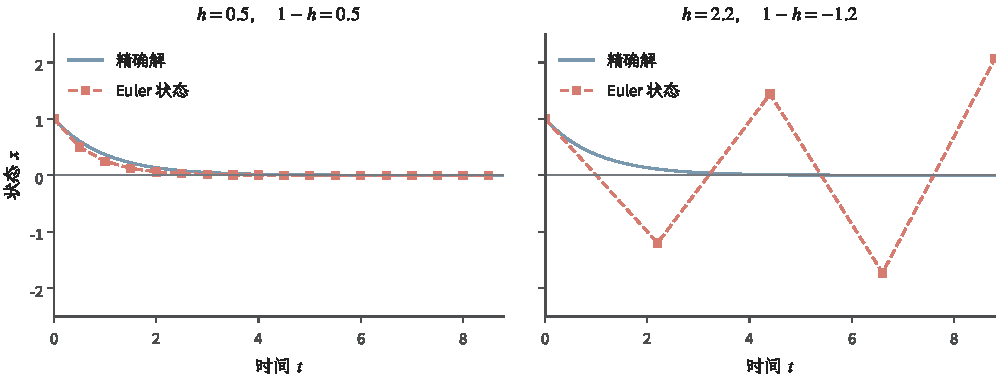
\includegraphics[width=\linewidth]{figures/01-mathematical-preliminaries/05-dynamical-systems-control-decision-and-games/matplotlib/dynamics/euler-stability.pdf}
  \caption{教学方程$\dot x=-x$、$x(0)=1$的精确解与Euler近似。蓝色实线为精确解，
  红色方点为数值状态；左图$h=0.5$衰减，右图$h=2.2$交替增长。两图采用相同坐标
  范围，连线只连接相邻数值状态。右图的发散来自步长，并非原连续系统不稳定。}
  \label{fig:dynamical-euler-stability}
\end{figure*}

\subsubsection{线性状态下的精确离散}

一般方法近似一步流，线性方程则可在规定的输入模型下直接积分。设
$[t_n,t_n+h)$内$\bm u(t)=\bm u_n$，对
式~\eqref{eq:dynamical-lti-variation-constants}取一个区间，得到
\begin{align}
  \bm x_{n+1}&=\bm A_h\bm x_n+\bm B_h\bm u_n,
    \label{eq:dynamical-zoh-discrete}\\
  \bm A_h&=\mathrm e^{h\bm A},\qquad
  \bm B_h=\int_0^h\mathrm e^{(h-s)\bm A}\bm B\,\mathrm ds.
    \label{eq:dynamical-zoh-matrices}
\end{align}
这称为\term{零阶保持}离散化。精确性针对区间内保持不变的输入，不表示真实输入
在区间内任意变化时也精确。若$\bm A$可逆，
$\bm B_h=\bm A^{-1}(\mathrm e^{h\bm A}-\bm I)\bm B$；$\bm A$奇异时继续使用积分
形式，不人为引入不存在的逆。输入保持误差与计算矩阵指数的数值误差仍可能存在，
只是没有Euler式的时间截断误差。

\subsubsection{保守状态下的几何离散}

对于可分Hamilton量，势能子系统保持位置、只改变动量；动能子系统保持动量、
只改变位置。两者各自可精确求解，因而可用对称分裂组成一步蛙跳：
\begin{align}
  \bm p_{n+1/2}&=\bm p_n-\frac h2\nabla U(\bm q_n),
    \label{eq:dynamical-leapfrog-half-momentum}\\
  \bm q_{n+1}&=\bm q_n+h\bm M^{-1}\bm p_{n+1/2},
    \label{eq:dynamical-leapfrog-position}\\
  \bm p_{n+1}&=\bm p_{n+1/2}-\frac h2\nabla U(\bm q_{n+1}).
    \label{eq:dynamical-leapfrog-final-momentum}
\end{align}
它是“动量半步、位置整步、动量半步”，不是把两条方程各做一次独立Euler更新。
令
$S_U^c(\bm q,\bm p)=(\bm q,\bm p-c\nabla U(\bm q))$、
$S_K^h(\bm q,\bm p)=(\bm q+h\bm M^{-1}\bm p,\bm p)$。
若$U\in C^2$，相应Jacobian为
\[
  \bm G_U=\begin{bmatrix}\bm I&\bm0\\-c\nabla^2U&\bm I\end{bmatrix},
  \qquad
  \bm G_K=\begin{bmatrix}\bm I&h\bm M^{-1}\\\bm0&\bm I\end{bmatrix}.
\]
三角结构使二者行列式均为$1$；$\nabla^2U$和$\bm M^{-1}$的对称性又给出
$\bm G_U^\top\bm J\bm G_U=\bm J$及
$\bm G_K^\top\bm J\bm G_K=\bm J$。故复合
$\Psi_h=S_U^{h/2}\circ S_K^h\circ S_U^{h/2}$保持体积且为辛映射。

每个子步换成负步长便是其逆，三步的对称排列使
$\Psi_h^{-1}=\Psi_{-h}$。若$R(\bm q,\bm p)=(\bm q,-\bm p)$是动量翻转，则还有
\[
  R\circ\Psi_h\circ R=\Psi_{-h}=\Psi_h^{-1}.
\]
因此这里的时间反演关系涉及动量翻转。把同一个映射连续应用两次便回到原态，
即$\Psi_h\circ\Psi_h=\operatorname{id}$，才称该映射为对合（involution）；
上面的逆映射关系不要求$\Psi_h$满足这个条件。
在足够光滑和固定有限时域下，蛙跳具有二阶全局精度。合适光滑性、轨迹有界及
小步长条件下的修正能量分析解释了常见的长时间有界能量振荡；辛性本身不保证
原Hamilton量每步完全相同。

\begin{example}[谐振子的精确与数值轨道]
  \label{ex:dynamical-harmonic-oscillator}
  取$U(q)=q^2/2,M=1$，精确解沿$q^2+p^2$的等值圆运动。蛙跳一步为
  \[
    \begin{bmatrix}q_{n+1}\\p_{n+1}\end{bmatrix}
    =
    \begin{bmatrix}1-h^2/2&h\\-h+h^3/4&1-h^2/2\end{bmatrix}
    \begin{bmatrix}q_n\\p_n\end{bmatrix}.
  \]
  更新矩阵的行列式为$1$、迹为$2-h^2$。当$0<h<2$时，其特征值是不同的
  单位模共轭数，并精确保持
  $(1-h^2/4)q_n^2+p_n^2$；这是一族椭圆，不是原来的能量圆。
  例如从$(1,0)$出发取$h=1$，一步得到$(1/2,-3/4)$，
  原能量从$1/2$变成$13/32$，却仍保持上述修正二次型。
  $h>2$时出现模大于$1$的特征值，$h=2$时还有退化导致的增长方向。
\end{example}
所以可逆、辛、体积保持与数值稳定分别需要检查。将这类轨迹用于随机采样时，
能量误差还需接受校正，不能把几何积分器直接当作精确采样器。

\subsection{仿射更新下的轨迹并行计算}

离散化选择数值规则，并行计算则重新安排同一规则的求值。对仿射递推
\begin{equation}
  \bm x_{t+1}=\bm A_t\bm x_t+\bm b_t,
  \label{eq:dynamical-affine-recurrence}
\end{equation}
用二元组$g_t=(\bm A_t,\bm b_t)$表示一步，定义较晚更新接在较早更新之后的复合为
\begin{equation}
  (\bm A_2,\bm b_2)\circ(\bm A_1,\bm b_1)
  =(\bm A_2\bm A_1,\bm A_2\bm b_1+\bm b_2).
  \label{eq:dynamical-affine-composition}
\end{equation}
复合结果仍是同维度仿射映射，这是能够紧凑表示整段更新的关键。三步直接核对得
\[
  \begin{aligned}
    g_3\circ(g_2\circ g_1)
    &=(\bm A_3\bm A_2\bm A_1,\,
       \bm A_3\bm A_2\bm b_1+\bm A_3\bm b_2+\bm b_3)\\
    &=(g_3\circ g_2)\circ g_1.
  \end{aligned}
\]
结合律允许用前缀扫描（prefix scan）同时求全部$g_{t-1}\circ\cdots\circ g_0$。
把更新按时间次序放在一棵平衡二叉树的叶子上，上行阶段合并相邻块，
每个内部节点保存自己整段的总复合。这个阶段只得到块的总映射，
全部中间状态还需要一次下传。

下传时，节点接收其区间之前已经完成的累计映射$p$。
左孩子继续接收$p$；若左块的总映射是$L$，右孩子就接收$L\circ p$。
根节点接收恒等映射$(\bm I,\bm0)$。例如四步$g_0,g_1,g_2,g_3$时，
左半块的总映射为$L=g_1\circ g_0$，四个叶子接收到的前缀分别是
\[
 \begin{aligned}
 p_0&=\operatorname{id},&p_1&=g_0,\\
 p_2&=L,&p_3&=g_2\circ L.
 \end{aligned}
\]
叶子$i$再形成$g_i\circ p_i$并作用于$\bm x_0$，便得到$\bm x_{i+1}$。
右块始终接在左块之后，所以这套下传规则也适用于不交换的复合。

总工作量统计所有节点执行的合并次数，计算深度统计最长依赖链上的合并次数。
$T$步形成的平衡树有$O(T)$个节点、$O(\log T)$层，
上下两阶段在每个节点只做常数次合并，同层互不依赖的节点可同时计算。
因此把一次固定维度合并视为一个操作时，总工作量为$O(T)$，深度为$O(\log T)$。
矩阵维度增长时，合并的实际算术成本仍需另算。

扫描保留时间次序。若$g_1(\bm x)=\operatorname{diag}(2,1)\bm x$、
$g_2(\bm x)=\bm x+(1,0)^\top$，则
\[
  (g_2\circ g_1)(\bm0)=(1,0)^\top,\qquad
  (g_1\circ g_2)(\bm0)=(2,0)^\top.
\]
这两个结果说明结合律不能换成交换律。浮点运算下，改变括号也可能改变舍入结果，
尤其是长乘积或条件数较大的传播；并行实现应按误差容限验证，而不是要求逐位相同。
若$\bm A_t,\bm b_t$只依赖事先给定的输入，仍可预先组成仿射扫描；若依赖尚未
算出的状态，或复合后不再有固定大小的封闭表示，就需要另行分析，不能直接套用。

\section{状态轨迹的极限与稳定}
\label{sec:dynamical-stability-sensitivity}

轨迹最终接近哪里，与小扰动会造成多大偏离，不是同一个问题。稳定方程可能在中途
放大误差，守恒轨迹也可能始终不接近任何一点。以下先统一这些性质的含义，再依据
线性或非线性结构选择判据。数值递推若另有步长误差，应把它作为另一个系统分析。

\subsection{状态轨迹的极限与稳定性质}

\begin{definition}[平衡点与稳定性]
  \label{def:dynamical-equilibrium-stability}
  考虑局部Lipschitz自治方程$\dot{\bm x}=\bm f(\bm x)$。
  满足$\bm f(\bm x^\star)=\bm0$的状态称为平衡点。以下性质均要求所涉及初值的
  解对全部$t\geq0$存在。

  平衡点在Lyapunov意义下\term{稳定}，是指对每个$\varepsilon>0$，存在
  $\delta>0$，使$\|\bm x(0)-\bm x^\star\|<\delta$蕴含
  $\|\bm x(t)-\bm x^\star\|<\varepsilon$对全部$t\geq0$成立。
  它具有局部吸引性，是指存在$r>0$，使所有
  $\|\bm x(0)-\bm x^\star\|<r$的解都趋于$\bm x^\star$。
  同时稳定且有局部吸引性称为\term{渐近稳定}。
  若存在$r,C,\alpha>0$，对上述$r$邻域内全部初值和$t\geq0$都有
  \[
    \|\bm x(t)-\bm x^\star\|_2
    \leq C\mathrm e^{-\alpha t}\|\bm x(0)-\bm x^\star\|_2,
  \]
  则称为局部指数稳定。若同一估计对全部初值成立，则称为全局指数稳定。
\end{definition}
离散时间把$t\geq0$换成非负整数，平衡条件换成
$F(\bm x^\star)=\bm x^\star$，指数因子可写成$q^t$，其中$0<q<1$。
“最终接近”与“始终不远离”分别对应吸引与稳定；不能只展示一条收敛轨迹，
便省去邻域内全部初值的量词。指数条件还要求$C,\alpha$在整个邻域统一。

\begin{table*}[htbp]
  \centering
  \begin{tabularx}{\linewidth}{lXXX}
    \toprule
    方程与原点 & 小初值始终小 & 轨迹趋于原点 & 统一指数衰减\\
    \midrule
    $\dot x=0$ & 是，状态保持初值 & 否，非零初值不动 & 否\\
    $\dot x=-x^3$ & 是，$|x(t)|$不增 & 是，代数衰减 & 否\\
    $\dot x=-x$ & 是 & 是 & 是，$|x(t)|=\mathrm e^{-t}|x(0)|$\\
    \bottomrule
  \end{tabularx}
  \caption{零输入下原点的稳定性质。第二行的解为
  $x(t)=x(0)/\sqrt{1+2x(0)^2t}$，它回到原点但不具有统一指数速度。
  三种方程均有全局解，比较不涉及数值离散。}
  \label{tab:dynamical-stability-types}
\end{table*}

有些轨迹不趋于一点，而是长期绕着一个集合运动。对此需要集合版本的描述。
\begin{definition}[不变集合与轨迹极限集]
  \label{def:dynamical-invariant-limit-sets}
  设$\Phi_t$是局部Lipschitz自治方程的流，并要求所述集合上的解正向全局存在。
  若$\Phi_t(\Omega)\subseteq\Omega$对全部$t\geq0$成立，则$\Omega$为
  \term{正向不变集}。若$\Phi_t(M)=M$对全部$t\geq0$成立，则$M$为
  \term{不变集}；这还要求集合内每一点有任意长时间以前的集合内前像，等价于
  每点都位于始终留在集合内的完整轨迹上。
  对正向有界轨迹，定义其\term{$\omega$极限集}为
  \[
    \omega(\bm x_0)=
    \{\bm z:\text{存在 }t_j\to\infty\text{ 使 }\bm x(t_j)\to\bm z\}.
  \]
\end{definition}
正向不变集限制一批初值的全部未来，极限集则记录一条轨迹在越来越晚的时刻反复
靠近的状态。趋于集合指到该集合的距离趋零，不要求在集合内部停止运动。

为了不逐条求解轨迹，常寻找一个能度量离开平衡点程度的标量。以原点为平衡，
$V\in C^1(D)$若满足$V(\bm0)=0$且非零点上$V>0$，称为正定的Lyapunov候选。
“候选”只说明它有合适的空间形状，还没有证明沿轨迹的变化方向。
\begin{definition}[Lyapunov函数]
  \label{def:dynamical-lyapunov-function}
  对$\dot{\bm x}=\bm f(\bm x)$，若上述正定候选还满足
  $\dot V(\bm x):=\nabla V(\bm x)^\top\bm f(\bm x)\leq0$，
  则称其为该邻域内的\term{Lyapunov函数}；若非零点处严格小于零，
  则称为严格Lyapunov函数。
\end{definition}
它不必等于物理能量。离散方程相应检查
$V(F(\bm x))-V(\bm x)$。正定性使“小能量”确实限制所有状态方向，
非增性才保证轨迹不能穿越更高的能量边界。下面的线性与非线性判据共同使用这两项。

\subsection{线性演化下的轨迹稳定性}

\subsubsection{长期演化的谱判据}

离散齐次系统为
\begin{equation}
  \bm x_{t+1}=\bm A\bm x_t,\qquad \bm x_t=\bm A^t\bm x_0.
  \label{eq:dynamical-discrete-linear-homogeneous}
\end{equation}
矩阵的幂、Jordan分解与指数已在第~\ref{chap:matrix-analysis}章建立。这里用它们
把长期轨迹问题化成谱的位置。
\begin{theorem}[离散线性系统的渐近稳定性]
  \label{thm:dynamical-discrete-spectral-stability}
  式~\eqref{eq:dynamical-discrete-linear-homogeneous}的原点全局渐近稳定，
  当且仅当$\rho(\bm A)=\max_{\lambda\in\operatorname{spec}(\bm A)}|\lambda|<1$。
  在此条件下，原点实际上全局指数稳定。
\end{theorem}
\begin{proof}
  在复数域写$\bm A=\bm V\bm J\bm V^{-1}$。大小为$r$的Jordan块
  $\bm J_\lambda=\lambda\bm I+\bm N$满足
  \[
    \bm J_\lambda^t
      =\sum_{j=0}^{\min(t,r-1)}\binom tj\lambda^{t-j}\bm N^j.
  \]
  $\lambda=0$的块在有限步后为零；$0<|\lambda|<1$时，多项式因子被几何衰减
  压过。取$\rho(\bm A)<q<1$，全部有限个块可统一控制为$Cq^t$，乘回换基矩阵
  得$\|\bm A^t\|\leq C' q^t$。它既给出趋零，也给出稳定性所需的统一有界增益。
  反之，若存在$|\lambda|\geq1$，沿其特征向量的复轨迹不趋零；分解成实部与虚部，
  至少一条实轨迹不趋零。单位模特征值的非平凡Jordan块还可能多项式增长。
  故渐近稳定要求全部特征值严格在单位圆内。
\end{proof}

\begin{theorem}[连续线性系统的指数稳定性]
  \label{thm:dynamical-continuous-spectral-stability}
  系统$\dot{\bm x}=\bm A\bm x$的原点全局指数稳定，当且仅当$\bm A$的全部
  特征值实部严格为负。这样的矩阵称为Hurwitz矩阵。
\end{theorem}
\begin{proof}
  对Jordan块，
  $\mathrm e^{t(\lambda\bm I+\bm N)}
   =\mathrm e^{\lambda t}\sum_{j=0}^{r-1}t^j\bm N^j/j!$。
  若全部实部为负，取$0<\alpha<-\max_\lambda\operatorname{Re}\lambda$，
  有限次多项式乘指数可统一控制为$C\mathrm e^{-\alpha t}$。乘回换基矩阵就得到
  $\|\mathrm e^{t\bm A}\|\leq C'\mathrm e^{-\alpha t}$。
  若某个特征值实部非负，则对应实不变子空间中存在增长、常值或不衰减振荡的轨迹，
  不可能满足该指数界。非平凡Jordan块不会消除这种障碍。
\end{proof}
连续系统检查左半平面，离散系统检查单位圆。边界上的谱需另查Jordan结构：
可能稳定而不吸引，也可能增长，不能把严格不等号改成非严格不等号。

谱给出长期方向，二次能量给出一个可逐时刻检查的证书。取
$V(\bm x)=\bm x^\top\bm P\bm x$，其中$\bm P\succ\bm0$，则
\begin{equation}
  \dot V=\bm x^\top(\bm A^\top\bm P+\bm P\bm A)\bm x.
  \label{eq:dynamical-continuous-lyapunov-derivative}
\end{equation}
\begin{theorem}[线性Lyapunov方程]
  \label{thm:dynamical-linear-lyapunov-equation}
  $\bm A$为Hurwitz矩阵，当且仅当对每个$\bm Q\succ\bm0$，存在唯一
  $\bm P\succ\bm0$满足
  \begin{equation}
    \bm A^\top\bm P+\bm P\bm A=-\bm Q.
    \label{eq:dynamical-continuous-lyapunov-equation}
  \end{equation}
\end{theorem}
\begin{proof}
  若$\bm A$为Hurwitz矩阵，定义
  $\bm P=\int_0^\infty\mathrm e^{t\bm A^\top}\bm Q\mathrm e^{t\bm A}\,\mathrm dt$。
  指数稳定保证积分收敛。任意非零$\bm x$对应的被积二次型非负，且在$t=0$
  严格为正，所以$\bm P\succ\bm0$。对被积矩阵求导并积分，得
  \[
    \bm A^\top\bm P+\bm P\bm A
    =[\mathrm e^{t\bm A^\top}\bm Q\mathrm e^{t\bm A}]_0^\infty=-\bm Q.
  \]
  两解之差$\bm D$满足$\bm A^\top\bm D+\bm D\bm A=\bm0$，故
  $\mathrm e^{t\bm A^\top}\bm D\mathrm e^{t\bm A}$恒为$\bm D$；
  令$t\to\infty$得$\bm D=\bm0$。

  反之，若存在正定的$\bm P,\bm Q$满足方程，记
  $p_-=\lambda_{\min}(\bm P)$、$p_+=\lambda_{\max}(\bm P)$、
  $q_-=\lambda_{\min}(\bm Q)$。则
  $p_-\|\bm x\|_2^2\leq V\leq p_+\|\bm x\|_2^2$，且
  $\dot V=-\bm x^\top\bm Q\bm x\leq-(q_-/p_+)V$。
  乘以积分因子得到
  \[
    \|\bm x(t)\|_2
    \leq\sqrt{p_+/p_-}\,
      \mathrm e^{-q_-t/(2p_+)}\|\bm x(0)\|_2.
  \]
  这直接证明指数稳定；由已证谱判据，$\bm A$为Hurwitz矩阵。
\end{proof}
反向证明只用二次型上下界与积分估计，不依赖尚未建立的非线性判据。

\begin{theorem}[离散时间Lyapunov方程]
  \label{thm:dynamical-discrete-lyapunov-equation}
  $\rho(\bm A)<1$，当且仅当对每个$\bm Q\succ\bm0$，存在唯一
  $\bm P\succ\bm0$满足$\bm A^\top\bm P\bm A-\bm P=-\bm Q$。
\end{theorem}
\begin{proof}
  正向取
  $\bm P=\sum_{j=0}^\infty(\bm A^\top)^j\bm Q\bm A^j$。
  上述离散指数界使级数绝对收敛；首项正定、其余项半正定，故$\bm P$正定。
  左乘$\bm A^\top$、右乘$\bm A$后相减即得方程。两解之差满足
  $\bm D=(\bm A^\top)^t\bm D\bm A^t$，令$t\to\infty$得唯一性。
  反向用$V(\bm x)=\bm x^\top\bm P\bm x$，有
  \[
    V(\bm A\bm x)-V(\bm x)=-\bm x^\top\bm Q\bm x<0
    \quad(\bm x\neq\bm0).
  \]
  比值$V(\bm A\bm x)/V(\bm x)$在单位球面上连续且严格小于$1$，
  因紧性有统一上界$c<1$，且$c\geq0$。于是$V(\bm x_t)\leq c^t V(\bm x_0)$
  （$c=0$时一步后即为零）。二次型界给出指数稳定，再由谱判据得到$\rho(\bm A)<1$。
\end{proof}
线性系统因此总能为稳定动力学找到某个二次能量，但这个能量一般不是欧氏范数平方。
下一项正说明更换度量为什么重要。

\subsubsection{有限时间的瞬态放大}

取
\[
  \bm A=\begin{bmatrix}1/2&K\\0&1/2\end{bmatrix},\qquad K>0.
\]
无论$K$多大，谱半径均为$1/2$，而
\[
  \bm A^t=
  \begin{bmatrix}
    2^{-t}&tK\,2^{-(t-1)}\\0&2^{-t}
  \end{bmatrix}.
\]
从$\bm x_0=(0,1)^\top$出发，第一步即为$(K,1/2)^\top$，欧氏范数可以大幅
增长；之后$t2^{-t}\to0$才使状态趋零。这里放大来自第二坐标向第一坐标的耦合，
没有任何输入或数值误差。

\begin{figure}[htbp]
  \centering
  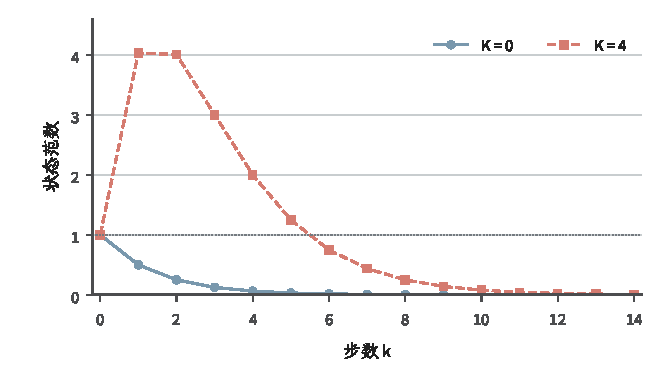
\includegraphics[width=\linewidth]{figures/01-mathematical-preliminaries/05-dynamical-systems-control-decision-and-games/matplotlib/concepts-dynamics/transient-growth.pdf}
  \caption{同谱系统的不同瞬态。初值均为$(0,1)^\top$，蓝色圆点取$K=0$，
  红色方点取$K=4$，谱半径均为$1/2$。后者前两步范数约为$4.03$、$4.01$，
  随后才趋零；灰线为初始范数$1$。长期衰减不等于每一步都收缩。}
  \label{fig:dynamical-transient-growth}
\end{figure}

$K\neq0$时，$\bm A^\top\bm A\neq\bm A\bm A^\top$，矩阵非正规。
本例只有一个独立特征向量，幂零耦合产生$t2^{-t}$项；可对角化但特征向量近乎
共线的非正规矩阵，也可能因模态先相消、后分离而放大。有限时间增益
$\|\bm A^t\|$、伪谱与合适的Lyapunov范数描述了谱半径以外的信息。
谱稳定没有许诺欧氏范数下逐步收缩，更没有许诺中间状态不越过任务边界。

\subsection{非线性演化下的轨迹稳定性}

\subsubsection{平衡邻域内的稳定判据}

非线性系统一般无法通过一个固定矩阵构造全局二次能量，因而需要寻找候选函数。
它可以来自物理能量、误差平方或模型特有的守恒与耗散关系。找到候选以后，
仍须检查正定性、沿轨迹导数以及适用区域。\scite{math-khalil2002nonlinear}
\begin{theorem}[连续时间Lyapunov判据]
  \label{thm:dynamical-nonlinear-lyapunov}
  设原点为$\dot{\bm x}=\bm f(\bm x)$的平衡点，$\bm f$在其邻域内局部Lipschitz。
  若该邻域存在$C^1$正定候选$V$且$\dot V\leq0$，则原点稳定；
  若非零点上$\dot V<0$，则原点局部渐近稳定。
  若这些条件在$\mathbb R^d$上成立，且$V(\bm x)\to\infty$当
  $\|\bm x\|\to\infty$，则所有解正向全局存在；非增情形给出稳定性，
  严格下降情形给出全局渐近稳定性。
\end{theorem}
\begin{proof}
  选足够小的$\varepsilon$使闭球位于适用邻域。球面上的连续正函数$V$有
  最小值$c_\varepsilon>0$。原点处连续性给出$\delta<\varepsilon$，
  使$\|\bm x_0\|<\delta$时$V(\bm x_0)<c_\varepsilon$。
  轨迹若首次触及球面，必须达到至少$c_\varepsilon$的能量，与$\dot V\leq0$
  矛盾。更具体地，可选$\bm x_0$所在的闭子水平集与闭球的交作为紧集$K$，
  且其能量水平严格低于球面最小值；轨迹不能穿出$K$，局部解可延拓到任意正时间。
  对全部足够小$\varepsilon$得到此结论即为稳定性。

  若$\dot V$在非零点严格为负，反设某条上述轨迹不趋零，则存在$\varepsilon_0>0$
  及$t_j\to\infty$，使$\|\bm x(t_j)\|\geq\varepsilon_0$。
  在紧集$K$上令$M=\sup_K\|\bm f\|$。非零轨迹下可取$M>0$；
  速度有界使每次达到该半径后至少在长度$\varepsilon_0/(2M)$内保持
  $\|\bm x\|\geq\varepsilon_0/2$。函数$-\dot V$在
  $K\cap\{\|\bm x\|\geq\varepsilon_0/2\}$上有严格正下界。
  选取互不相交的这些时间段，能量便减少无穷大量，与$V\geq0$矛盾。
  因而轨迹趋零。全局且径向无界时，每个初值的子水平集都紧；
  同样的延拓与下降论证适用于任意初值，得到全局结论。
\end{proof}
径向无界性控制的是远处状态，不能用“在原点附近正定”代替。
若还能找到$c_1,c_2,c_3>0$使
$c_1\|\bm x\|^2\leq V\leq c_2\|\bm x\|^2$、$\dot V\leq-c_3\|\bm x\|^2$，
则前述线性方程证明中的积分估计同样给出局部指数衰减。一般严格负导数未必有
这种二次型比较，所以渐近稳定未必指数稳定。

\subsubsection{不变区域内的极限集合}

机械能常只在某些方向上直接耗散，导致$\dot V=0$的集合远大于平衡点。
这时应问：轨迹能否一直留在这个集合中？LaSalle原理把这个问题转成极限集合判据。
\begin{theorem}[LaSalle不变性原理]
  \label{thm:dynamical-lasalle-invariance}
  设自治向量场$\bm f$局部Lipschitz，$\Omega$紧且正向不变，
  $V$在包含$\Omega$的开邻域上为$C^1$，并有$\dot V\leq0$。
  令$E=\{\bm x\in\Omega:\dot V(\bm x)=0\}$，$M$为$E$中最大不变集，
  则从$\Omega$出发的每条轨迹满足
  $\operatorname{dist}(\bm x(t),M)\to0$。
\end{theorem}
\begin{proof}
  紧性排除有限时间逃逸，也使$\omega(\bm x_0)$非空且紧。
  沿轨迹的$V$单调不增且有下界，故趋于$v_\infty$。
  对极限点$\bm z=\lim_j\bm x(t_j)$，连续性给出$V(\bm z)=v_\infty$。

  对固定$s\geq0$，流的初值连续性使
  $\bm x(t_j+s)\to\Phi_s(\bm z)$，故
  $\Phi_s(\omega(\bm x_0))\subseteq\omega(\bm x_0)$。
  反过来，充分大的$j$有$t_j>s$。紧性允许从$\bm x(t_j-s)$取收敛子列，
  其极限$\bm w$属于$\omega(\bm x_0)$，且$\Phi_s(\bm w)=\bm z$。
  因此$\Phi_s(\omega(\bm x_0))=\omega(\bm x_0)$，这里得到的是完整不变性，
  而非仅正向不变性。

  $V$在极限集上恒为$v_\infty$，从其中任一点出发的轨迹仍在该集合，
  所以沿轨迹导数为零。于是$\omega(\bm x_0)$是$E$内的不变集，必包含于$M$。
  若到$M$的距离不趋零，就有$\varepsilon>0$及$t_j\to\infty$使距离至少为
  $\varepsilon$。紧性再给出收敛子列，其极限属于$\omega(\bm x_0)\subseteq M$，
  与此距离下界矛盾。
\end{proof}

\begin{example}[阻尼振子的零导数集合]
  \label{ex:dynamical-damped-oscillator-lasalle}
  对$\dot q=p,\dot p=-q-cp$，其中$c>0$，取$V=(q^2+p^2)/2$，则
  $\dot V=q p+p(-q-cp)=-cp^2\leq0$。
  零导数集合为$p=0$；但其上$q\neq0$的点满足$\dot p=-q\neq0$，
  马上离开该直线。因此零导数集合中最大不变集只有原点。
  每个能量子水平集均紧且正向不变，LaSalle原理遂给出所有轨迹趋于原点。
\end{example}

\begin{figure}[htbp]
  \centering
  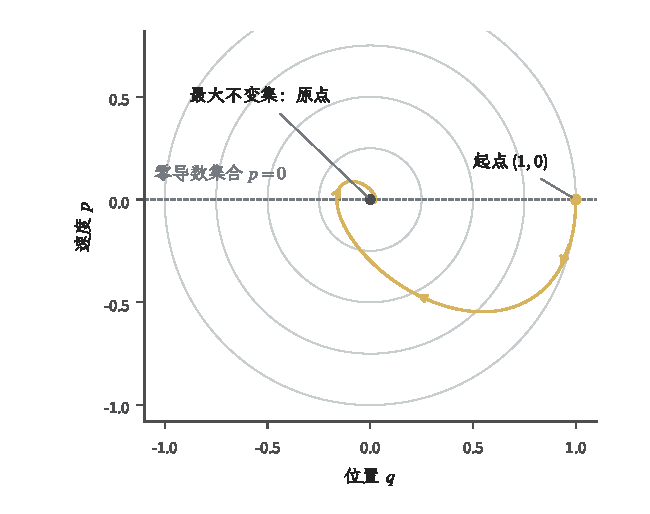
\includegraphics[width=\linewidth]{figures/01-mathematical-preliminaries/05-dynamical-systems-control-decision-and-games/matplotlib/teaching-dynamics/lasalle-zero-set.pdf}
  \caption{阻尼振子$\dot q=p,\dot p=-q-p$从$(1,0)$出发的精确轨迹。
  黄色轨迹覆盖$t=0$至$12$，箭头指示时间；灰色虚线为$\dot V=0$的直线$p=0$，
  浅灰圆为能量参考等值线。起点虽在零导数集合上，初始速度$(0,-1)$却将它带离
  该集合；能一直留在其中的完整轨迹只有原点。}
  \label{fig:reader-lasalle-zero-set}
\end{figure}
能量非增先限制活动区域，动力学再排除不能持续停留的零导数点。
把整个$E$直接称为“最终状态”，会丢掉LaSalle论证中最关键的一步。

\subsection{初值与输入扰动下的轨迹稳定性}

前述原点判据通常对应零输入，或把恒定输入下的平衡平移到原点。
温度例的恒定$u_t=0.4$对应平衡$2$，误差$e_t=x_t-2$才满足$e_{t+1}=0.8e_t$。
不能因为误差趋零，就说实际温度趋于环境温度。

对连续方程，若$\bm f$关于状态具有Lipschitz常数$L$，同一输入下两条解满足
\[
  \|\bm x(t)-\widetilde{\bm x}(t)\|
  \leq \mathrm e^{L(t-t_0)}\|\bm x_0-\widetilde{\bm x}_0\|.
\]
这是由积分方程与引理~\ref{lem:action-state-gronwall}得到的有限时间连续依赖，
在$L>0$时没有声称衰减。若输入也不同、$\bm f$关于输入的Lipschitz常数为$L_u$，
并且比较模型沿第二条轨迹还有大小至多$r(s)$的向量场误差，则同一引理给出
\[
  \|\bm x(t)-\widetilde{\bm x}(t)\|
  \leq \mathrm e^{L(t-t_0)}\|\bm x_0-\widetilde{\bm x}_0\|
  +\int_{t_0}^t\mathrm e^{L(t-s)}
     \bigl(L_u\|\bm u(s)-\widetilde{\bm u}(s)\|+r(s)\bigr)\,\mathrm ds.
\]
初态误差、输入误差、模型误差因此有不同来源，却都要经过后续动态传播。

对指数稳定线性系统，若
$\|\mathrm e^{t\bm A}\|\leq M\mathrm e^{-\alpha t}$，常数变易公式给出更强的界：
\[
  \|\bm x(t)\|
  \leq M\mathrm e^{-\alpha(t-t_0)}\|\bm x_0\|
  +M\|\bm B\|\int_{t_0}^t\mathrm e^{-\alpha(t-s)}\|\bm u(s)\|\,\mathrm ds.
\]
若$\|\bm u(s)\|\leq U$，第二项至多
$(M\|\bm B\|U/\alpha)(1-\mathrm e^{-\alpha(t-t_0)})$。
有界输入产生有界状态，但持续输入通常留下非零稳态。
离散温度例若输入固定偏多$\delta u$，稳态偏差就是
$\delta u/(1-0.8)=5\delta u$。稳定性消退初值记忆，不会自动消除持续施加的偏差。

\section{随机状态与随机轨迹}
\label{sec:dynamical-ito-fokker-planck}

给定相同初温与加热量，开门、风速等未显式建模的作用仍可能改变真实温度。
把这些作用表示成过程噪声后，更新公式不再只产生一条确定轨迹，而是把噪声的联合
规律转换为状态的联合规律。本节只研究这种生成机制，尚未用任何传感器读数条件化。
离散更新可以直接逐步随机生成；连续时间必须先说明随机增量怎样累计。

\subsection{随机状态的离散演化}

\subsubsection{随机递推与状态转移}

在同一概率空间上给定初始状态、输入及背景随机量，写
\[
  \bm x_{t+1}=F_t(\bm x_t,\bm u_t,\bm\varepsilon_{t+1}).
\]
若$\bm\varepsilon_{t+1}$独立于已有状态历史，分布为$\nu_{t+1}$，且$F_t$可测，
并将本节的输入$(\bm u_t)$固定为预先给定的确定序列，则由更新映射得到转移核
\[
  K_t(\bm x,A)=\int
    \mathbb I\{F_t(\bm x,\bm u_t,\bm e)\in A\}\,\nu_{t+1}(\mathrm d\bm e).
\]
对每个$\bm x$它是概率分布，对每个可测$A$它关于$\bm x$可测，符合
定义~\ref{def:probability-kernel}。独立性使
$\mathbb P(\bm x_{t+1}\in A\mid\bm x_{0:t})=K_t(\bm x_t,A)$，
这才得到当前状态的Markov性质。给定$\pi_0=\mathcal L(\bm x_0)$，整条有限轨迹满足
\[
  \mathbb P(\bm x_{0:T}\in\mathrm d\bm z_{0:T})
  =\pi_0(\mathrm d\bm z_0)
    \prod_{t=0}^{T-1}K_t(\bm z_t,\mathrm d\bm z_{t+1}),
\]
其中乘积表示逐次核积分。它同时规定跨时刻依赖，而不只是各个时刻的边缘分布。
若以后改用仅依赖当前状态的可测反馈$\bm u_t=\pi_t(\bm x_t)$，
把$\pi_t(\bm x)$代入核即可。若输入还依赖更早的状态或带噪观测，
仅有新噪声独立通常不足以使$\bm x_t$本身为Markov状态；
须保留相应历史或扩充状态。这一区别将在
第~\ref{chap:control-theory}章“策略的实现与轨迹控制”中用于规定可实施策略。

常用的线性加性模型为
\begin{equation}
  \bm x_{t+1}=\bm A_t\bm x_t+\bm B_t\bm u_t+\bm w_{t+1}.
  \label{eq:dynamical-linear-state-model}
\end{equation}
若$\bm w_{t+1}\sim\mathcal N(\bm0,\bm Q_{t+1})$且独立于初态与其他过程噪声，
$K_t(\bm x,\cdot)=\mathcal N(\bm A_t\bm x+\bm B_t\bm u_t,\bm Q_{t+1})$。
即便$\bm Q_{t+1}$奇异，它仍是合法概率核，只是不一定有全维Lebesgue密度。

相关噪声需要重新检查条件结构。例如
$x_{t+1}=a x_t+w_{t+1}$，而$w_{t+1}=\rho w_t+\varepsilon_{t+1}$，
其中新$\varepsilon$独立。代入$w_t=x_t-a x_{t-1}$得
$x_{t+1}=(a+\rho)x_t-\rho a x_{t-1}+\varepsilon_{t+1}$。
一般仅给$x_t$已不足够；可把$(x_t,w_t)$扩成状态，或保留对更长历史的条件依赖。
“递推里有噪声”不等于“当前状态是Markov的”。

温度模型现在恢复为
\[
  x_{t+1}=0.8x_t+u_t+w_{t+1},\qquad
  w_{t+1}\sim\mathcal N(0,0.04).
\]
取各$w_t$相互独立且独立于初态。若$x_0=0,u_t=0.4$，
则$\mathbb E x_t=2(1-0.8^t)$，过程方差为
$0.04\sum_{j=0}^{t-1}0.8^{2j}$。平均轨迹仍与无噪模型相同，一条实际轨迹却会
在其附近波动。图~\ref{fig:action-state-temperature-layers}再叠加
$y_t=x_t+v_t$、$v_t\sim\mathcal N(0,0.09)$的独立读数噪声，
先展示生成层次；怎样由读数推断状态留到观测部分。

\begin{figure*}[htbp]
  \centering
  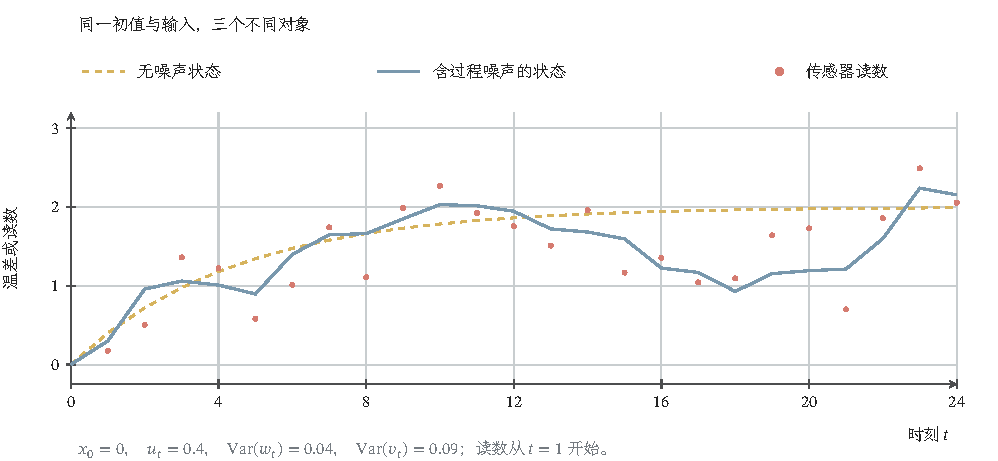
\includegraphics[width=\linewidth]{figures/01-mathematical-preliminaries/05-dynamical-systems-control-decision-and-games/tikz/dynamics/temperature-state-observation.pdf}
  \caption{同一温度模型的三个对象。初态$x_0=0$，输入始终为$0.4$；
  无噪声轨迹趋于$2$，过程噪声改变真实状态，独立观测噪声又把真实状态变成带噪读数。
  噪声方差分别为$0.04$和$0.09$。图中带噪曲线是固定种子的教学模拟，
  不是置信区间，也没有把读数用于反向校正状态。}
  \label{fig:action-state-temperature-layers}
\end{figure*}

\subsubsection{单时间尺度的随机逼近}
\label{sec:stoch-approximation-markov-noise}

有些递推状态不是房间温度，而是希望逐步求出的参数。设未知均值为$\mu$，
目标是解平均方程
\begin{equation}
  h(\theta)=\mathbb E[Y-\theta]=\mu-\theta=0.
  \label{eq:stoch-mean-root}
\end{equation}
每次只能得到一个含噪观测，仍可沿观测建议的方向作小步移动。这就是
\term{随机逼近}：用随机逐步更新寻找平均漂移的根，或其稳定不变对象。
算法轮次以括号上标标记，区别于物理状态的时间下标。
一般形式为
\begin{equation}
  \bm\theta^{(t+1)}=\bm\theta^{(t)}+\alpha_t
   [\overline{\bm h}(\bm\theta^{(t)})+\bm\xi_{t+1}+\bm r_{t+1}],
  \label{eq:stoch-general-stochastic-approximation}
\end{equation}
其中$\alpha_t>0$是步长，$\overline{\bm h}$是平均漂移，
$\mathbb E[\bm\xi_{t+1}\mid\mathcal F_t]=\bm0$是鞅差噪声，
$\bm r_{t+1}$记录近似、截断或尚未平衡所致的偏差。
Markov观测一般不能直接作为这个鞅差，稍后将分解其累计误差。

均值问题的Robbins--Monro递推为
\begin{equation}
  \theta^{(t+1)}=\theta^{(t)}
       +\alpha_t(Y_{t+1}-\theta^{(t)}).
  \label{eq:stoch-robbins-monro-mean}
\end{equation}
观测高于当前估计就上移，低于估计就下移。若
$\mathbb E[Y_{t+1}\mid\mathcal F_t]=\mu$，条件平均方向恰为$\mu-\theta^{(t)}$。
取$\alpha_t=1/(t+1)$时，第一步完全采用$Y_1$；归纳得
$\theta^{(t)}=t^{-1}\sum_{s=1}^tY_s$。一般步长对应不等权的递推，
所以随机逼近不限于样本平均。\scite{math-robbins1951stochastic}

经典递减步长条件是
\begin{equation}
  \sum_{t=0}^\infty\alpha_t=\infty,\qquad
  \sum_{t=0}^\infty\alpha_t^2<\infty.
  \label{eq:stoch-robbins-monro-stepsizes}
\end{equation}
前者保留无限的累计移动能力；若鞅差噪声的条件二阶矩有统一上界，
后者就能控制累计的加权方差。具体地，对此前信息$\mathcal F_t$和鞅差$\xi_{t+1}$，
若$\mathbb E[\xi_{t+1}^2\mid\mathcal F_t]\leq\sigma^2$，则
\[
 \sum_{t=0}^\infty\alpha_t^2
 \mathbb E[\xi_{t+1}^2\mid\mathcal F_t]
 \leq\sigma^2\sum_{t=0}^\infty\alpha_t^2<\infty.
\]
仅有每个时刻的方差有限还不够，因为这些方差可能随时间无界增长。
$\alpha_t=c/(t+t_0)^\gamma$在$c,t_0>0$、$1/2<\gamma\leq1$时满足两项。
若步长和有限，初始误差可能尚未消除就停止有效移动；若平方和无穷，
上述噪声控制不再适用，但这本身也不是任意模型必然发散的断言。

固定步长则保留持续响应新数据的能力。对独立同分布、均值$\mu$、方差$\sigma^2$
的观测，确定初值及$\alpha_t=\alpha\in(0,1)$给出
\[
  e_{t+1}=(1-\alpha)e_t+\alpha(Y_{t+1}-\mu),\qquad
  \mathbb E e_t=(1-\alpha)^t e_0.
\]
由独立性，方差$v_{t+1}=(1-\alpha)^2v_t+\alpha^2\sigma^2$，因而
\[
  v_t=\frac{\alpha\sigma^2}{2-\alpha}
       [1-(1-\alpha)^{2t}]
  \longrightarrow\frac{\alpha\sigma^2}{2-\alpha}.
\]
初始偏差消失，随机波动却留下正的稳态方差。小步长降低此误差，也延缓对初值或
目标变化的响应。这是固定均值模型的精确计算，不能替代一般非线性递推的稳定证明。

\begin{figure*}[htbp]
  \centering
  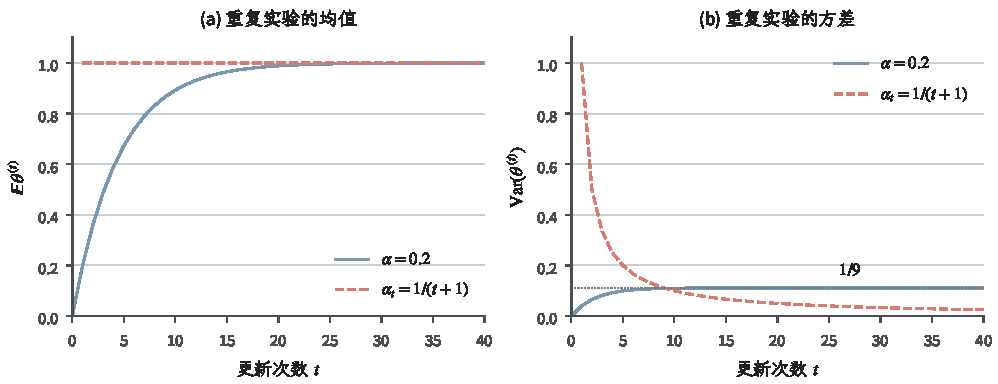
\includegraphics[width=\linewidth]{figures/01-mathematical-preliminaries/05-dynamical-systems-control-decision-and-games/matplotlib/concepts-probability/stochastic-stepsize-bias-variance.pdf}
  \caption{同一均值问题的重复实验均值与方差。取$\theta^{(0)}=0,\mu=1,\sigma^2=1$，
  观测独立同分布；蓝实线为固定$\alpha=0.2$，红虚线为$\alpha_t=1/(t+1)$。
  固定步长方差趋于$1/9$，样本平均方差为$1/t$。曲线由解析式得到，不是一条样本轨迹。}
  \label{fig:stochastic-stepsize-bias-variance}
\end{figure*}

要把“噪声越来越小”变成逐路径收敛，需要控制累计噪声，而不只计算单步均值。
下面保留一个可完整证明的代表性结论。
\begin{lemma}[带可求和误差的非负超鞅]
  \label{lem:stoch-almost-supermartingale}
  设$Z_t,A_t$为关于$\mathcal F_t$的非负可积适应过程，$b_t\geq0$为确定数，
  且$\mathbb E[Z_{t+1}\mid\mathcal F_t]\leq Z_t-A_t+b_t$。
  若$\sum_tb_t<\infty$，则$Z_t$几乎必然收敛到有限随机变量，
  且$\sum_tA_t<\infty$几乎必然成立。
\end{lemma}
\begin{proof}
  令$r_t=\sum_{s=t}^\infty b_s$、$U_t=Z_t+r_t$。因为$r_t=b_t+r_{t+1}$，
  有$\mathbb E[U_{t+1}\mid\mathcal F_t]\leq U_t-A_t$。
  $U_t$是非负超鞅，由非负超鞅收敛定理几乎必然收敛到有限值。
  取期望并累加得到
  $\mathbb E\sum_{t=0}^nA_t\leq\mathbb E U_0$。
  单调收敛给出$\mathbb E\sum_{t=0}^\infty A_t\leq\mathbb E U_0<\infty$，
  所以该非负级数几乎必然有限。又$r_t\to0$，故$Z_t=U_t-r_t$也收敛。
\end{proof}
其中的鞅与超鞅收敛工具见第~\ref{chap:stochastic-processes-and-approximation}章；
本引理把可求和误差吸收到一个真正的超鞅中。

\begin{theorem}[均值求根的几乎必然收敛]
  \label{thm:stoch-mean-root-convergence}
  设$\mathcal F_t$包含$\theta^{(0)},Y_1,\ldots,Y_t$，且
  $\mathbb E[(\theta^{(0)}-\mu)^2]<\infty$。若
  \[
    \mathbb E[Y_{t+1}\mid\mathcal F_t]=\mu,\qquad
    \mathbb E[(Y_{t+1}-\mu)^2\mid\mathcal F_t]\leq\sigma^2,
  \]
  步长满足式~\eqref{eq:stoch-robbins-monro-stepsizes}并最终有$0<\alpha_t\leq1$，
  则式~\eqref{eq:stoch-robbins-monro-mean}的$\theta^{(t)}\to\mu$几乎必然成立。
\end{theorem}
\begin{proof}
  记$e_t=\theta^{(t)}-\mu$、$\xi_{t+1}=Y_{t+1}-\mu$，则
  $e_{t+1}=(1-\alpha_t)e_t+\alpha_t\xi_{t+1}$。
  初值与条件二阶矩假设递归保证每个有限时刻的$\mathbb E e_t^2$有限。
  舍去有限前缀，令$0<\alpha_t\leq1$。条件展开平方，交叉项为零，得到
  \[
    \mathbb E[e_{t+1}^2\mid\mathcal F_t]
    =(1-\alpha_t)^2e_t^2
      +\alpha_t^2\mathbb E[\xi_{t+1}^2\mid\mathcal F_t]
    \leq e_t^2-\alpha_te_t^2+\alpha_t^2\sigma^2.
  \]
  对移位序列应用前一引理，取$Z_t=e_t^2,A_t=\alpha_te_t^2$、
  $b_t=\alpha_t^2\sigma^2$。可积性与可求和条件均已核对，故$e_t^2$几乎必然
  收敛，且$\sum_t\alpha_te_t^2<\infty$。
  若某条样本路径的极限为$L>0$，最终就有$e_t^2\geq L/2$，
  从而$\sum_t\alpha_te_t^2\geq(L/2)\sum_t\alpha_t=\infty$，矛盾。
  所以$L=0$，得到结论。
\end{proof}
平方可和控制噪声，步长和发散排除残留误差。若条件均值有不可忽略偏差，
或条件方差失控，证明中的递推不等式就失去依据。向量非线性情形还须控制迭代
有界性，不能把标量结论仅通过换粗体符号推广。

一般漂移适合在与步长匹配的时钟上观察。定义算法时间
\begin{equation}
  \tau_0=0,\qquad \tau_t=\sum_{s=0}^{t-1}\alpha_s,
  \label{eq:stoch-algorithmic-time}
\end{equation}
并在相邻$(\tau_t,\bm\theta^{(t)})$之间线性插值为$\widehat{\bm\theta}(\tau)$。
对应平均ODE是
\begin{equation}
  \dot{\bm\theta}(\tau)=\overline{\bm h}(\bm\theta(\tau)).
  \label{eq:stoch-mean-ode}
\end{equation}
\term{ODE方法}不是说每个随机增量都等于平均增量，而是要求任意固定算法时间窗
上的累计随机偏差最终消失。一个常用的接口是：$\alpha_t\to0$、
$\sum_t\alpha_t=\infty$，$\overline{\bm h}$局部Lipschitz，迭代几乎必然有界，
并对每个$H>0$有
\[
  \sup_{\substack{k\geq t\\\tau_k-\tau_t\leq H}}
  \left\|\sum_{s=t}^{k-1}\alpha_s(\bm\xi_{s+1}+\bm r_{s+1})\right\|
  \longrightarrow0\quad\text{几乎必然}.
\]
在这些条件下，插值的积分方程相对平均ODE只剩一个在有限窗上一致趋零的残差。
局部Lipschitz与有界性给出该窗口上的统一常数，应用
引理~\ref{lem:action-state-gronwall}，便得到插值与从同一晚期状态出发的ODE
轨迹在该窗上一致接近。这一步连接的是有限窗轨迹；再结合平均ODE的全局渐近
稳定平衡及紧集上的吸引性，才能得到迭代收敛到该平衡。\scite{math-borkar2008stochastic}

对均值根，平均方程及其解为
\begin{equation}
  \dot\theta=\mu-\theta,\qquad
  \theta(\tau)=\mu+(\theta(0)-\mu)\mathrm e^{-\tau}.
  \label{eq:stoch-mean-root-ode-solution}
\end{equation}
取$V=(\theta-\mu)^2/2$则$\dot V=-(\theta-\mu)^2$，与前述误差平方证明一致。
一般系统可能有多个吸引子；平均稳定不意味着全局最优。迭代有界性也须证明，
例如建立远处负漂移的径向无界函数。投影到紧凸集虽可强制有界，却改变了边界上的
平均动力学；不能把所得极限不加论证地叫作原方程的根，或原根的欧氏投影。

现在转向相关观测。固定核$P$、平稳分布$\pi$，随机更新为$H(\theta,Z_t)$时，
平均漂移是
\begin{equation}
  \overline h(\theta)=\int H(\theta,z)\,\pi(\mathrm dz).
  \label{eq:stoch-markov-mean-field}
\end{equation}
即使$Z_t$已平稳，$H(\theta,Z_t)-\overline h(\theta)$给定过去也未必均值为零。
需要把相关误差转成可控制的鞅和边界项。
\begin{definition}[Markov核的Poisson方程]
  \label{def:stoch-markov-poisson-equation}
  固定$P,\pi$与$\pi$可积的$H(\theta,\cdot)$。若可测函数$g_\theta$满足
  \begin{equation}
    g_\theta(z)-Pg_\theta(z)=H(\theta,z)-\overline h(\theta),
    \qquad Pg_\theta(z)=\int g_\theta(z')P(z,\mathrm dz'),
    \label{eq:stoch-poisson-equation}
  \end{equation}
  且所用积分有限，则称其为相应\term{Poisson方程}的解。
\end{definition}
这里的Poisson方程属于Markov算子，不是随后用于事件噪声的Poisson计数过程。
若链对历史满足$\mathcal L(Z_{t+1}\mid\mathcal F_t)=P(Z_t,\cdot)$，相关变量可积，
则
\begin{align}
  H(\theta,Z_t)-\overline h(\theta)
    &=g_\theta(Z_t)-g_\theta(Z_{t+1})+\Delta M_{t+1}(\theta),
       \label{eq:stoch-poisson-decomposition}\\
  \Delta M_{t+1}(\theta)&=g_\theta(Z_{t+1})-Pg_\theta(Z_t).\notag
\end{align}
最后一项给定$\mathcal F_t$均值为零；前两项固定参数时会望远镜消去。
参数与步长变化时还剩余项，不能直接把它们删掉。

\begin{lemma}[固定有限链的加权Poisson分解]
  \label{lem:stoch-finite-chain-poisson-sum}
  设$P$为固定的有限不可约非周期核，参数递推
  $\theta^{(t+1)}=\theta^{(t)}+\alpha_tH(\theta^{(t)},Z_t)$始终位于紧集$K$，
  $H$在$K$上一致有界且关于参数一致Lipschitz。若正步长单调递减并满足
  式~\eqref{eq:stoch-robbins-monro-stepsizes}，且链对所用历史具有上述条件转移核，
  则
  $\sum_{t=0}^n\alpha_t[H(\theta^{(t)},Z_t)-\overline h(\theta^{(t)})]$
  几乎必然收敛。特别地，任意向晚期移动的有限算法时间窗上的尾和趋零。
\end{lemma}
\begin{proof}
  记$q_\theta=H(\theta,\cdot)-\overline h(\theta)$。
  有限不可约非周期链几何收敛，且$\pi q_\theta=0$，所以
  $g_\theta=\sum_{j=0}^\infty P^jq_\theta$绝对一致收敛，并满足
  $g_\theta-Pg_\theta=q_\theta$。
  对$q_\theta-q_{\theta'}$应用相同几何界，得到有限常数$G,L_g$使
  $|g_\theta(z)|\leq G$、
  $|g_\theta(z)-g_{\theta'}(z)|\leq L_g|\theta-\theta'|$。

  加权鞅和$\sum_{t=0}^n\alpha_t\Delta M_{t+1}(\theta^{(t)})$的条件方差和被
  $4G^2\sum_t\alpha_t^2$控制，因而在$L^2$中有界并几乎必然收敛。
  剩余项从$m$到$n$作分部求和，得到
  \begin{align*}
    &\sum_{t=m}^n\alpha_t
       [g_{\theta^{(t)}}(Z_t)-g_{\theta^{(t)}}(Z_{t+1})]\\
    &\quad=\alpha_mg_{\theta^{(m)}}(Z_m)
       -\alpha_ng_{\theta^{(n)}}(Z_{n+1})\\
    &\qquad+\sum_{t=m+1}^n
       [\alpha_tg_{\theta^{(t)}}(Z_t)
        -\alpha_{t-1}g_{\theta^{(t-1)}}(Z_t)].
  \end{align*}
  中间每项绝对值至多
  $G(\alpha_{t-1}-\alpha_t)
    +\alpha_{t-1}L_g|\theta^{(t)}-\theta^{(t-1)}|$。
  有界更新给出$|\theta^{(t)}-\theta^{(t-1)}|\leq C\alpha_{t-1}$。
  第一部分由单调性望远镜求和，第二部分由平方可和控制，端点因$\alpha_t\to0$
  而消失。故剩余级数也收敛，与鞅和相加即得结论。收敛级数的任意尾区间和一致
  趋零，自然包含固定算法时间长度对应的索引窗。
\end{proof}

例~\ref{ex:stoch-two-state-chain}中的链取值$0,2$，平稳均值$\mu=2/3$，
且$P(z-\mu)=0.7(z-\mu)$。对$H(\theta,z)=z-\theta$，可取
$g_\theta(z)=(z-\mu)/(1-0.7)=\frac{10}{3}(z-\mu)$。
它恰好不依赖参数，因此参数变化余项也消失。Poisson分解没有把相关样本变成独立
样本，而是重新组织累计误差。

一般状态空间要另外证明Poisson解存在、具有所需矩界且随参数规则变化。
若$Z_{t+1}\sim P_{\bm\theta^{(t)}}(Z_t,\cdot)$，则平均漂移也变成
$\overline{\bm h}(\bm\theta)=\int\bm H(\bm\theta,z)\pi_{\bm\theta}(\mathrm dz)$，
相应方程为$g_{\bm\theta}-P_{\bm\theta}g_{\bm\theta}
=H(\bm\theta,\cdot)-\overline h(\bm\theta)$。
每个固定参数下分别遍历并不够：算法不断改变参数，需要在访问区域上统一控制
混合速度、Poisson解的矩及参数Lipschitz界，再控制参数变化造成的加权余项。
统一几何遍历、适当的矩界与联合有界性是常见充分条件。
它们使相关波动在算法时间上可忽略，不能把不稳定的平均根变成稳定根。

\subsubsection{双时间尺度的随机逼近}
\label{sec:action-state-two-timescale}

一个参数可能负责快速跟踪另一个参数尚未解释的误差，另一个参数则慢慢改变目标。
此时采用两个更新时钟：
\begin{align*}
  \bm u^{(t+1)}
    &=\bm u^{(t)}+\beta_t[
        \bm g(\bm u^{(t)},\bm v^{(t)})+\bm\eta_{t+1}+\bm r^u_{t+1}],\\
  \bm v^{(t+1)}
    &=\bm v^{(t)}+\alpha_t[
        \bm f(\bm u^{(t)},\bm v^{(t)})+\bm\xi_{t+1}+\bm r^v_{t+1}].
\end{align*}
这里$\bm u^{(t)},\bm v^{(t)}$是算法变量，不是贯穿温度模型的行动与读数。
两组步长都满足Robbins--Monro条件，且$\alpha_t/\beta_t\to0$时，
$\bm u$相对较快，$\bm v$相对较慢。例如
$\beta_t=(t+1)^{-0.6}$、$\alpha_t=(t+1)^{-0.9}$满足尺度分离。

快时间上把$\bm v$暂时固定，得到
$\dot{\bm u}=\bm g(\bm u,\bm v)$；若其稳定平衡为$\bm u^\star(\bm v)$，
慢时间上再使用
$\dot{\bm v}=\bm f(\bm u^\star(\bm v),\bm v)$。
一组常用的充分条件是：漂移局部Lipschitz；快平衡对每个慢状态全局渐近稳定，
其吸引性在所访问的紧参数区域上一致，且平衡映射局部Lipschitz；约化慢ODE有
全局渐近稳定平衡$\bm v^\star$；联合迭代几乎必然有界；两组鞅差的条件二阶矩
在访问区域有统一界，残差在各自有限算法时间窗上可忽略。在这些条件与步长条件下，
标准双时间尺度结论给出
$(\bm u^{(t)},\bm v^{(t)})\to
(\bm u^\star(\bm v^\star),\bm v^\star)$。\scite{math-borkar2008stochastic}
Markov背景则需在两个时钟上分别验证相应的Poisson与统一混合条件。

\begin{example}[分解同一个未知均值的快慢更新]
  \label{ex:stoch-two-timescale-mean-splitting}
  若$\mathbb E[Y_{t+1}\mid\mathcal F_t]=\mu$，取
  \[
    u^{(t+1)}=u^{(t)}+\beta_t(Y_{t+1}-u^{(t)}-v^{(t)}),\qquad
    v^{(t+1)}=v^{(t)}+\alpha_t(u^{(t)}-v^{(t)}).
  \]
  冻结$v$后，快方程$\dot u=\mu-v-u$的唯一稳定平衡为$u^\star(v)=\mu-v$。
  代入慢方程得$\dot v=\mu-2v$，于是$v^\star=\mu/2$，
  $u^\star(v^\star)=\mu/2$。快变量估计尚未被$v$解释的部分，慢变量调整两部分
  的分配。若再满足两组步长条件、统一有界的条件噪声方差、有限二阶矩初值以及
  联合迭代几乎必然有界，则上述条件给出联合收敛。
\end{example}
尺度分离没有保证快平衡存在，也没有保证其稳定或全局最优。两组步长同阶时，
该线性例仍可用联合系统分析，却不能继续使用冻结慢变量的论证。
此外，这里的噪声增量是$\alpha_t\xi_{t+1}$，方差尺度为$\alpha_t^2$；
后面扩散模拟的增量为$\sqrt h\,\xi$，方差尺度为$h$。
平均ODE中噪声在有限算法时间窗消失，SDE中噪声则保留有限二次变差，两者不能互换。

\subsubsection{平均动力学的稳定判据}
\label{sec:dynamical-mean-dynamics-linear-recursion}

现在只检查前两项中的平均方向，步长与噪声条件继续使用已建立的接口。线性平均漂移
常写为
\begin{equation}
  \overline{\bm h}(\bm\theta)=\bm b-\bm A\bm\theta.
  \label{eq:dynamical-linear-mean-drift}
\end{equation}
若$\bm A$可逆，平衡为$\bm\theta^\star=\bm A^{-1}\bm b$，误差满足
\begin{equation}
  \dot{\bm e}=-\bm A\bm e.
  \label{eq:dynamical-linear-mean-error-ode}
\end{equation}
稳定性检查$-\bm A$是否Hurwitz，即$\bm A$的特征值实部是否为正。
负号不可漏掉。$\bm A$也未必是某个损失的Hessian，不能仅凭更新外形套用凸性。

对一般实矩阵，反对称部分的二次型为零，因而
$\bm e^\top\bm A\bm e=\bm e^\top(\bm A+\bm A^\top)\bm e/2$。
若
\begin{equation}
  \frac{\bm A+\bm A^\top}{2}\succ\bm0,
  \label{eq:dynamical-positive-symmetric-part}
\end{equation}
则欧氏能量$V=\|\bm e\|_2^2/2$严格下降，给出方便的充分条件。
它不是必要条件：$\bm A=\left[\begin{smallmatrix}1&10\\0&1\end{smallmatrix}\right]$
的特征值均为$1$，而对称部分
$\left[\begin{smallmatrix}1&5\\5&1\end{smallmatrix}\right]$有负特征值。
平均误差仍指数稳定，只是欧氏范数可能暂时增大。只要$-\bm A$为Hurwitz矩阵，
线性Lyapunov方程便为任意$\bm Q\succ\bm0$给出$\bm P\succ\bm0$满足
\begin{equation}
  \bm A^\top\bm P+\bm P\bm A=\bm Q.
  \label{eq:dynamical-mean-drift-lyapunov}
\end{equation}
此时$V=\bm e^\top\bm P\bm e$的导数为$-\bm e^\top\bm Q\bm e$，
加权几何吸收了非对称耦合。

时序差分（temporal difference, TD）更新提供了一个具体来源。
固定只依赖当前状态的行动规则$\pi$后，设有限状态$S_t$按转移矩阵$\bm P_\pi$演化，
每步收益$R_{t+1}$按当前转移产生，其规律不随时间改变且绝对值有界。
取$0\leq\gamma<1$，从状态$i$出发的收益价值定义为
\[
 v_\pi(i)=\mathbb E_i^\pi
 \left[\sum_{k=0}^\infty\gamma^kR_{k+1}\right].
\]
这里近似的是累计收益的期望，不是某一次随机实现；
下标$i$表示把初态固定为$i$，几何级数保证这个期望有限。
拆出第一步，并按下一状态作条件平均，便有
\[
 v_\pi(i)=\mathbb E_i^\pi[R_1+\gamma v_\pi(S_1)].
\]
用特征$\bm\phi(i)\in\mathbb R^q$的线性组合$\bm\phi(i)^\top\bm\theta$近似$v_\pi(i)$，
再以样本转移$i\to j$及收益$R$替代这个条件平均，便得到更新方向
$\bm\phi(i)[R+\gamma\bm\phi(j)^\top\bm\theta-\bm\phi(i)^\top\bm\theta]$。
它用当前值与“一步收益加下一状态值”的差纠正参数。
令平稳访问概率为$\bm d$、$\bm D=\operatorname{diag}(\bm d)$，
$\bm\Phi$的第$i$行为$\bm\phi(i)^\top$，
在同一策略的平稳访问下平均得到
\begin{equation}
  \overline{\bm h}(\bm\theta)=\bm b-\bm A_{\mathrm{TD}}\bm\theta,\qquad
  \bm A_{\mathrm{TD}}=\bm\Phi^\top\bm D
                    (\bm I-\gamma\bm P_\pi)\bm\Phi.
  \label{eq:dynamical-td-mean-matrix}
\end{equation}
若$r_i=\mathbb E[R\mid i]$，则$\bm b=\bm\Phi^\top\bm D\bm r$。
固定策略的求值关系在这里解释非对称平均矩阵的来源，策略的选择则留给
第~\ref{chap:policy-value-and-optimization}章。该章主要按成本计价，
把本例收益取负即可转换到相应的成本价值约定。

先设所考虑状态的$d_i>0$，以便
$\|\bm z\|_{\bm D}=(\bm z^\top\bm D\bm z)^{1/2}$为范数。
Jensen不等式给出$(\bm P_\pi\bm z)_i^2\leq\sum_j(P_\pi)_{i,j}z_j^2$；
乘$d_i$求和，并用平稳性$\sum_id_i(P_\pi)_{i,j}=d_j$，得到
\begin{equation}
  \|\bm P_\pi\bm z\|_{\bm D}\leq\|\bm z\|_{\bm D}.
  \label{eq:dynamical-markov-contraction-weighted}
\end{equation}
再由Cauchy--Schwarz，
$\langle\bm z,\bm P_\pi\bm z\rangle_{\bm D}\leq\|\bm z\|_{\bm D}^2$。
取$\bm z=\bm\Phi\bm c$，便有
\begin{align}
  \bm c^\top\bm A_{\mathrm{TD}}\bm c
    &=\|\bm\Phi\bm c\|_{\bm D}^2
       -\gamma\langle\bm\Phi\bm c,\bm P_\pi\bm\Phi\bm c\rangle_{\bm D}\notag\\
    &\geq(1-\gamma)\|\bm\Phi\bm c\|_{\bm D}^2.
    \label{eq:dynamical-td-positive-drift}
\end{align}
若$\bm\Phi^\top\bm D\bm\Phi\succ\bm0$，右侧对$\bm c\neq\bm0$严格为正，
所以平均矩阵的对称部分正定，具有唯一全局指数稳定平衡。
若允许$d_i=0$，加权量在全空间只是半范数，但上面的求和不等式仍成立；
严格结论仍须直接要求加权特征协方差正定，普通满列秩未必足够。
离策略采样改变访问权重而不同时改变目标转移，非扩张不等式可能失败，
故不能由此推出离策略稳定。

再用标量递推核对平均稳定与噪声条件怎样配合。设
$\theta^{(t+1)}=\theta^{(t)}+\alpha_t[b-a\theta^{(t)}+\xi_{t+1}]$，
$a>0$，噪声为条件均值零且条件二阶矩不超过$\sigma^2$，初值二阶矩有限。
令$e_t=\theta^{(t)}-b/a$，则
\[
  \mathbb E[e_{t+1}^2\mid\mathcal F_t]
  =(1-a\alpha_t)^2e_t^2+
       \alpha_t^2\mathbb E[\xi_{t+1}^2\mid\mathcal F_t].
\]
当$0<a\alpha_t\leq1$，右侧至多
$e_t^2-a\alpha_te_t^2+\alpha_t^2\sigma^2$。
应用已证几乎超鞅引理与两组步长级数，即得$e_t\to0$几乎必然；
在这个标量例中，论证本身给出路径有界性，无需额外假设。
固定步长则除要求$|1-a\alpha|<1$外，还会保留非零噪声方差。

快慢平均场也可逐个核对。考虑
\[
  y^{(t+1)}=y^{(t)}+\beta_t[x^{(t)}-y^{(t)}+\eta_{t+1}],\qquad
  x^{(t+1)}=x^{(t)}+\alpha_t[c-x^{(t)}-y^{(t)}+\xi_{t+1}].
\]
当$\alpha_t/\beta_t\to0$，冻结$x$得到快稳定根$y^\star(x)=x$；
代入慢场得到$\dot x=c-2x$，故候选联合极限为$(c/2,c/2)$。
它与前一个均值拆分例共享快慢逻辑，但更新方程不同。
上述代入仅核对了两个平均场；随机收敛仍须满足两组步长、噪声或Markov混合、
残差和联合有界性条件，不能由候选根直接替代整套论证。

\subsection{随机增量的积分累计}

离散更新只需说明每一步使用哪些已知量。把更新间隔缩到连续时间后，还须说明
被积系数在时间与随机结果的联合空间中是否可测。以下滤过
$(\mathcal F_t)_{t\geq0}$满足通常条件：$\mathcal F_0$包含概率零集的全部子集，
且$\mathcal F_t=\bigcap_{s>t}\mathcal F_s$。过程、滤过和停时的基础回见
第~\ref{chap:stochastic-processes-and-approximation}章。

一个过程$H$适应，表示每个$H_t$对$\mathcal F_t$可测。若对每个$T$，
$(t,\omega)\mapsto H_t(\omega)$在$[0,T]\times\Omega$上对
$\mathcal B([0,T])\otimes\mathcal F_T$可测，则称它渐进可测。
可预测过程则对由全部左连续适应过程生成的可预测$\sigma$代数可测。
这两项都包含时间方向的联合可测要求；逐时刻适应本身不够。
连续适应过程可预测；若$X$适应且路径右连续、有左极限，
则$X_{t-}$可预测，而跳跃后的$X_t$一般不能作为当次跳跃前已知的系数。

连续时间中也可以根据已经观察到的信息决定何时停止。
连续停时是取值于$[0,\infty]$的随机变量$\tau$，满足
$\{\tau\leq t\}\in\mathcal F_t$对每个实数$t\geq0$成立；
停止过程$M^\tau_t=M_{t\wedge\tau}$在到达$\tau$后保持当时的值。
若适应且右连续、有左极限的过程$M$存在递增停时$\rho_n\to\infty$几乎必然，
使每个$M^{\rho_n}$都是真鞅，就称$M$为局部鞅（local martingale）。
这里的“局部”是由随机停止限定的范围：每条路径最终能覆盖任意给定的有限时段，
却未保证去掉停止后仍能交换期望与极限。用这样的停止过程先证明结论、再逐步放开停止范围，称为局部化（localization）。

普通漂移的累计仍是逐路径的Lebesgue积分$\int_0^t b_s\,\mathrm ds$，
要求相应联合可测性及$\int_0^T|b_s|\,\mathrm ds<\infty$几乎必然。
噪声的累计规则则取决于增量类型：有限次跳跃可以逐事件相加，连续Brownian噪声
不能这样处理，也不能当作普通可积的时间导数。

\subsubsection{跳跃增量的积分}
\label{sec:action-state-poisson-integral}

令$N_t$为速率$\lambda>0$的Poisson计数过程，相对于共同滤过，
$N_t-N_s$独立于$\mathcal F_s$且服从$\operatorname{Pois}(\lambda(t-s))$。
记跳时为$\tau_1,\tau_2,\ldots$。有限活动指每个有界时间区间内几乎必然只有
有限个事件；它不要求整个无穷时间轴上事件总数有限。
对有限实值的可预测过程$H$，定义
\begin{equation}
  \int_0^t H_s\,\mathrm dN_s
    =\sum_{\tau_j\leq t}H_{\tau_j}.
  \label{eq:action-state-poisson-integral}
\end{equation}
若$H_s=g(s,X_{s-})$，第$j$个事件的贡献为$g(\tau_j,X_{\tau_j-})$。
事件已经发生后才知道的状态，不能反过来决定同一事件的可预测幅度。
上述和逐路径有定义；若还要交换期望与求和，需增加可积性。

对非负可预测$H$，Poisson补偿恒等式为
\[
  \mathbb E\int_0^T H_s\,\mathrm dN_s
       =\lambda\mathbb E\int_0^T H_s\,\mathrm ds.
\]
对简单过程$H_s=\sum_iH_i\mathbb I_{(t_i,t_{i+1}]}(s)$，
$H_i$对$\mathcal F_{t_i}$可测，等式由
$\mathbb E[H_i\Delta N_i]=\lambda\Delta t_i\mathbb E H_i$逐项相加得到。
非负简单可预测函数逼近与单调收敛把它推广到非负$H$；正负部均可积时推广到
有符号$H$。因此$\lambda\mathbb E\int_0^T|H_s|\,\mathrm ds<\infty$
保证跳跃和可积。

原计数同时包含平均增长与随机起伏。扣除平均增长，得到补偿计数
$\widetilde N_t=N_t-\lambda t$及积分
\begin{equation}
  \int_0^t H_s\,\mathrm d\widetilde N_s
    =\sum_{\tau_j\leq t}H_{\tau_j}
      -\lambda\int_0^t H_s\,\mathrm ds.
  \label{eq:action-state-compensated-poisson}
\end{equation}
若$\lambda\mathbb E\int_0^T H_s^2\,\mathrm ds<\infty$，
该过程为平方可积鞅，并满足
\begin{equation}
  \mathbb E\left|\int_0^T H_s\,\mathrm d\widetilde N_s\right|^2
       =\lambda\mathbb E\int_0^T H_s^2\,\mathrm ds.
  \label{eq:action-state-poisson-isometry}
\end{equation}
为核对这点，先取上述简单过程。每个$\Delta\widetilde N_i$在
$\mathcal F_{t_i}$条件下均值为零、方差为$\lambda\Delta t_i$。
对$i<j$，先在$\mathcal F_{t_j}$条件下求期望，便使
$H_i\Delta\widetilde N_iH_j\Delta\widetilde N_j$的期望为零。
平方展开只剩$\sum_i\lambda\Delta t_i\mathbb E H_i^2$。
同样的条件期望计算给出任意$s<t$间的鞅等式。
简单过程的二阶逼近、上述等距和条件期望的$L^2$连续性完成延拓；
补偿恒等式保证延拓与有限跳跃和表示一致。
若每个有限$T$上只有$\int_0^T H_s^2\,\mathrm ds<\infty$几乎必然，
可取
\[
 \rho_n=\inf\left\{t:\lambda\int_0^tH_s^2\,\mathrm ds\geq n\right\}\wedge n.
\]
累计平方是连续适应的非减过程，所以首次达到阈值可由当前历史判断，$\rho_n$为停时。
停止后的累计量不超过$n$，已证等距便保证相应补偿积分为平方可积鞅。
各有界区间的累计量有限又使$\rho_n\uparrow\infty$几乎必然，因此未停止的积分是局部鞅。
去掉停止时，逐路径收敛并不自动保留期望；还需例如固定时刻上停止变量族的一致可积性，才能据此得到零均值。

左极限不是无关紧要的记号。例如单位幅度事件有
\[
  \int_0^t N_{s-}\,\mathrm dN_s=\frac{N_t(N_t-1)}2,\qquad
  \sum_{\tau_j\leq t}N_{\tau_j}=\frac{N_t(N_t+1)}2.
\]
右侧第二个和使用了事件后的计数，两者相差$N_t$。
若错误地把$N_s$当作可预测系数，则
\[
  \mathbb E\left[\sum_{\tau_j\leq t}N_{\tau_j}
       -\lambda\int_0^t N_s\,\mathrm ds\right]=\lambda t\neq0.
\]
它不是声称的零均值补偿积分。用$N_{s-}$时，多出来的这一项恰好消失。

\subsubsection{连续增量的积分}

以下$\bm W$是在同一滤过下的$m$维标准Brownian运动，分量独立，
其增量独立于过去且协方差为时间长度乘$\bm I_m$。定义、路径性质以及
$[W^{(i)},W^{(j)}]_t=\delta_{i,j}t$回见
第~\ref{sec:dynamical-brownian-motion}节；本处只构造如何累计这些增量。
先用标量驱动，把可预测简单过程写为
$H_t=\sum_{i=0}^{n-1}H_i\mathbb I_{(t_i,t_{i+1}]}(t)$，
其中$0=t_0<\cdots<t_n=T$，$H_i\in L^2(\mathcal F_{t_i})$。
定义
\begin{equation}
  \int_0^T H_t\,\mathrm dW_t
       :=\sum_{i=0}^{n-1}H_i(W_{t_{i+1}}-W_{t_i}).
  \label{eq:dynamical-simple-ito-integral}
\end{equation}
系数可以依赖已发生的全部历史，但不能借用下一段增量。

记
$M_t=\sum_iH_i(W_{t\wedge t_{i+1}}-W_{t\wedge t_i})$。
对$s<t$，包含$s$的区间使用已知系数和$s$之后的零均值增量；
对起点$t_i\geq s$的后续区间，塔式性质给出
\[
  \mathbb E[H_i\Delta W_i\mid\mathcal F_s]
   =\mathbb E\{\mathbb E[H_i\Delta W_i\mid\mathcal F_{t_i}]
                  \mid\mathcal F_s\}=0.
\]
截断到$t$的最后一段同理。因此$\mathbb E[M_t\mid\mathcal F_s]=M_s$，
$M$是平方可积鞅，特别地$\mathbb E M_T=0$。
再核对平方：对$i<j$，$H_iH_j\Delta W_i$对$\mathcal F_{t_j}$可测，
故
\[
  \mathbb E[H_iH_j\Delta W_i\Delta W_j]=0,\qquad
  \mathbb E[H_i^2(\Delta W_i)^2]=\Delta t_i\,\mathbb E H_i^2.
\]
无界系数时可先截断再用$L^2$极限；交叉乘积由Cauchy--Schwarz保证可积。
逐项相加得到\term{Itô等距}：
\begin{equation}
  \mathbb E\left(\int_0^T H_t\,\mathrm dW_t\right)^2
       =\mathbb E\int_0^T H_t^2\,\mathrm dt.
  \label{eq:dynamical-ito-isometry}
\end{equation}
这与Poisson等距的推导结构相同，但此处尚没有逐路径的有限事件和。

对可预测$H$，若$\mathbb E\int_0^T H_t^2\,\mathrm dt<\infty$，
用简单可预测过程在该范数下逼近，等距关系使积分序列在$L^2$中为Cauchy序列，
从而定义与逼近选择无关的积分。条件期望是$L^2$压缩映射，故鞅性质保留；
所得鞅可取连续版本。渐进可测且平方可积的系数可在
$\mathbb P\otimes\mathrm dt$意义下取等价可预测版本，得到同一积分。
若每个有限$T$上只有$\int_0^T H_t^2\,\mathrm dt<\infty$几乎必然，则取
\[
 \rho_n=\inf\left\{t:\int_0^tH_s^2\,\mathrm ds\geq n\right\}\wedge n.
\]
这与Poisson积分的停止构造相同，只是不再乘速率$\lambda$。
停止后平方积分至多为$n$，所以可用Itô等距构造真鞅；
这些积分在共同的停止区间上一致，随$\rho_n\uparrow\infty$拼接成连续局部鞅。
矩阵系数逐分量积分时，等距右端改为Frobenius范数平方。

普通积分与Brownian积分的路径粗糙程度不同。路径$A$在$[0,T]$上有限变差
（finite variation），是指全部分割$\pi$上的绝对增量和有共同有限上界：
\[
 \operatorname{Var}_{[0,T]}(A)
 =\sup_\pi\sum_i|A_{t_{i+1}}-A_{t_i}|<\infty.
\]
这里求和的是绝对增量；二次变差则累计增量的平方，两者不是同一性质。
对$A_t=\int_0^t b_s\,\mathrm ds$，三角不等式给出
$\operatorname{Var}_{[0,T]}(A)\leq\int_0^T|b_s|\,\mathrm ds$，
因此漂移累计具有有限变差。向量情形可逐分量使用同一判断。
把漂移与Brownian累计合起来，就得到后面换元公式的对象。
\begin{definition}[连续Itô过程]
  \label{def:action-state-ito-process}
  设$\bm X_0$对$\mathcal F_0$可测，$\bm b_t$渐进可测，
  $\bm\sigma_t$可预测，且每个有限$T$上
  $\int_0^T(\|\bm b_t\|+\|\bm\sigma_t\|_{\mathrm F}^2)\,\mathrm dt<\infty$
  几乎必然。过程
  \[
    \bm X_t=\bm X_0+\int_0^t\bm b_s\,\mathrm ds
                         +\int_0^t\bm\sigma_s\,\mathrm d\bm W_s
  \]
  称为连续Itô过程。漂移积分有有限变差，随机积分是连续局部鞅。
\end{definition}
这里系数已经给定；若系数反过来依赖未知的$\bm X_t$，才形成待求解的方程。

积分约定可以由Brownian平方直接辨认：
\[
 W_{t_{i+1}}^2-W_{t_i}^2
     =2W_{t_i}\Delta W_i+(\Delta W_i)^2.
\]
求和并回用二次变差，左端点和趋于$(W_T^2-T)/2$，右端点和趋于
$(W_T^2+T)/2$。两者差$T$，不是随着网格变细就消失的误差。
连续半鞅是可分解为连续局部鞅与连续适应有限变差过程之和的过程；
前述Itô过程属于这一类。其二次协变差$[H,X]_t$由分割上
$\sum_i\Delta H_i\Delta X_i$的概率极限定义。
若$A$有限变差且$X$连续，交叉增量和满足
\[
 \left|\sum_i\Delta A_i\Delta X_i\right|
 \leq\max_i|\Delta X_i|\operatorname{Var}_{[0,T]}(A)
 \longrightarrow0.
\]
最后一步来自连续路径在紧区间上一致连续。因此这类因子与连续随机项的二次协变差为零，稍后线性方程的积分因子将使用这个性质。
对于连续半鞅$H,X$，
Stratonovich积分可定义为
\[
  \int_0^t H_s\circ\mathrm dX_s
       =\int_0^t H_s\,\mathrm dX_s+\tfrac12[H,X]_t.
\]
对本章的Itô过程，右侧积分按漂移与Brownian部分分别计算；
一般半鞅积分使用相应延拓。该定义对应对称端点和的概率极限。
在系数足够光滑的标量模型中，
$\mathrm dX=b_{\mathrm S}(X)\,\mathrm dt+\sigma(X)\circ\mathrm dW$
等价于Itô漂移$b_{\mathrm I}=b_{\mathrm S}+\sigma\sigma'/2$。
多维时修正为$\frac12\sum_j(D\bm\sigma_{\cdot j})\bm\sigma_{\cdot j}$。
Stratonovich形式保留普通链式法则，但不能只更换积分符号而不改漂移。
上述规则限定连续半鞅；跳跃换元要另外保留有限差。

\subsection{随机状态变换的Itô公式}

读数、能量和损失通常是状态的函数。已知状态怎样累计，怎样求这些函数的变化？
普通链式法则只保留一阶增量；连续随机增量的平方会累计为有限量，
一次跳跃又不能视为无穷小位移。这两种情形分别需要二阶修正与完整有限差。

\subsubsection{连续变化下的Itô公式}

\begin{theorem}[Itô公式]
  \label{thm:dynamical-ito-formula}
  设$\bm X$为定义~\ref{def:action-state-ito-process}中的过程，
  $f\in C^{1,2}([0,T]\times\mathbb R^d)$，即时间一阶、空间二阶偏导连续。
  则经局部化后，以概率$1$对所有$t$有下列积分等式；其微分记号为
  \begin{align}
    \mathrm df(t,\bm X_t)
      &=[\partial_t f+\nabla f^\top\bm b_t
         +\tfrac12\operatorname{tr}
               (\bm\sigma_t\bm\sigma_t^\top\nabla^2 f)]\,\mathrm dt\notag\\
      &\quad+\nabla f^\top\bm\sigma_t\,\mathrm d\bm W_t.
    \label{eq:dynamical-ito-formula}
  \end{align}
  各导数在$(t,\bm X_t)$取值。若要对等式直接取期望，还须漂移项可积，
  且随机被积项满足例如
  $\mathbb E\int_0^T\|\nabla f^\top\bm\sigma_t\|^2\,\mathrm dt<\infty$；
  局部鞅本身不保证期望为零。
\end{theorem}

先说明关键估计，以免把二阶项当作形式记忆规则。对有界连续适应系数，
局部化后的Taylor展开中，漂移平方和的期望为$O(|\pi|)$，
漂移与随机项乘积和的$L^1$范数为$O(|\pi|^{1/2})$；
这里$|\pi|$为分割的最大间距。这些项均消失。相反，对有界的
$\mathcal F_{t_i}$可测权重$c_i$，独立增量与正态四阶矩给出
\[
 \mathbb E\left|\sum_i c_i[(\Delta W_i)^2-\Delta t_i]\right|^2
   =2\sum_i\mathbb E[c_i^2](\Delta t_i)^2
   \leq2\sup_i\|c_i\|_\infty^2T|\pi|.
\]
不同Brownian分量的交叉乘积也以同样方式趋零。故加权平方项留下
时间积分，而不是零；矩阵写法恰为
$\operatorname{tr}(\bm\sigma\bm\sigma^\top\nabla^2f)/2$。

把$\Delta\bm X_i$中的系数冻结在左端点，也要控制误差。连续有界系数满足
\[
 \mathbb E\sum_i
 \left\|\int_{t_i}^{t_{i+1}}
    (\bm\sigma_s-\bm\sigma_{t_i})\,\mathrm d\bm W_s\right\|^2
 =\mathbb E\int_0^T
       \|\bm\sigma_s-\bm\sigma_{\lfloor s\rfloor_\pi}\|_{\mathrm F}^2\,\mathrm ds
 \longrightarrow0.
\]
漂移差用普通积分估计；一阶随机项用Itô等距控制。
在紧区域内，Hessian一致连续，空间Taylor余项的绝对值和至多为
$\omega(\max_i\|\Delta\bm X_i\|)\sum_i\|\Delta\bm X_i\|^2$，
其中$\omega(r)\to0$。路径连续使第一个因子趋零，第二个因子依上述估计
在概率上有界；余项因而依概率趋零。时间一阶项由$\partial_t f$的一致连续性处理。
这解释了光滑且系数连续有界时每类项的去向。

一般可测系数不能擅自用左端取样逼近。完整结果先按状态大小及累计可积量停时，
再以简单可预测过程逼近随机系数，并用连续局部鞅的二次协变差处理上述加权项，
最后令停时递增。这一一般化及$C^{1,2}$版本的完整证明见
Øksendal的随机微分方程教材第4章；上面的关键估计说明机制，不替代该一般证明。
\scite{math-oksendal2003sde}

例如$f(x)=x^2$给出
\[
  W_T^2=2\int_0^T W_s\,\mathrm dW_s+T,\qquad
  \int_0^T W_s\,\mathrm dW_s=(W_T^2-T)/2.
\]
常数系数则有$\int_0^T c\,\mathrm dW_s=cW_T$。
形式规则$(\mathrm dW)^2=\mathrm dt$、$\mathrm dt\,\mathrm dW=0$
总结了上述累计量级；它们不能替代可预测性与极限论证。

\subsubsection{跳跃变化下的Itô公式}
\label{sec:action-state-jump-ito}

考虑连续Itô部分加有限活动跳跃的右连续过程
\[
  \bm X_t=\bm X_0+\int_0^t\bm b_s\,\mathrm ds
        +\int_0^t\bm\sigma_s\,\mathrm d\bm W_s
        +\int_0^t\bm\gamma_s\,\mathrm dN_s,
\]
其中$\bm\gamma$可预测、在各事件处有限，$\bm b,\bm\sigma$满足前述局部
可积条件。对同样的$f\in C^{1,2}$，换元公式为
\begin{align}
 f(t,\bm X_t)-f(0,\bm X_0)
  ={}&\int_0^t[\partial_s f+\nabla f^\top\bm b_s
       +\tfrac12\operatorname{tr}(\bm\sigma_s\bm\sigma_s^\top\nabla^2f)]
                           (s,\bm X_{s-})\,\mathrm ds\notag\\
   &+\int_0^t\nabla f(s,\bm X_{s-})^\top\bm\sigma_s\,\mathrm d\bm W_s\notag\\
   &+\int_0^t[f(s,\bm X_{s-}+\bm\gamma_s)-f(s,\bm X_{s-})]\,\mathrm dN_s.
 \label{eq:action-state-jump-ito}
\end{align}
第一行中$\bm b_s,\bm\sigma_s$是过程系数，只把$f$的导数在所示点取值。
当跳跃次数与状态先被停时截断后，在相邻事件之间应用连续Itô公式，
到事件$\tau_j$处再加上精确增量
$f(\tau_j,\bm X_{\tau_j})-f(\tau_j,\bm X_{\tau_j-})$。
有限次相加，端点望远镜消去，即得此式。再去除截断，因有限活动与局部可积性，
得到每个有限时域上的结论。这一推导不需要把跳幅假设为很小。

若把$\nabla f^\top\mathrm d\bm X$统一写在前面，则还须显式加上
\[
 \sum_{\tau_j\leq t}
 [f(\tau_j,\bm X_{\tau_j})-f(\tau_j,\bm X_{\tau_j-})
          -\nabla f(\tau_j,\bm X_{\tau_j-})^\top\Delta\bm X_{\tau_j}].
\]
它不是只有二阶的近似，而是扣掉已计入一阶项后的全部有限差。
对补偿形式
$\mathrm d\bm X=\bm\beta_s\,\mathrm ds+\bm\sigma_s\,\mathrm d\bm W
                      +\bm\gamma_s\,\mathrm d\widetilde N$，
记$\Delta_\gamma f=f(s,\bm X_{s-}+\bm\gamma_s)-f(s,\bm X_{s-})$，
则$f$的漂移为
\[
 \partial_s f+\nabla f^\top\bm\beta_s
 +\tfrac12\operatorname{tr}(\bm\sigma_s\bm\sigma_s^\top\nabla^2f)
 +\lambda(\Delta_\gamma f-\nabla f^\top\bm\gamma_s),
\]
跳跃鞅项为$\Delta_\gamma f\,\mathrm d\widetilde N_s$。
由$\bm b=\bm\beta-\lambda\bm\gamma$及
$\mathrm dN=\mathrm d\widetilde N+\lambda\,\mathrm ds$代入即可核对；
取期望仍须检查该新被积项的可积性。

令$X=N$、$f(x)=x^2$，每次事件使平方增加$2N_{s-}+1$，所以
\[
  N_t^2=\int_0^t(2N_{s-}+1)\,\mathrm dN_s
       =2\int_0^tN_{s-}\,\mathrm d\widetilde N_s
         +\widetilde N_t+2\lambda\int_0^tN_s\,\mathrm ds+\lambda t.
\]
于是$\mathbb E N_t^2=(\lambda t)^2+\lambda t$。
Brownian平方的修正为连续的$t$，Poisson平方的修正为事件计数$N_t$；
后者再补偿才分成鞅与平均漂移。把两者都写成“噪声平方等于时间”会丢失事件信息。

\subsection{随机状态的连续演化}

至此我们能累计一个给定系数过程，也能计算其函数变化。状态模型还多一步：
下一段漂移和噪声幅度由当前未知状态决定，积分式因而成为关于整条轨迹的方程。
先明确方程与解，再检查成立条件，最后用线性结构实际求解。

\subsubsection{随机微分方程与积分表示}

\begin{definition}[Itô随机微分方程与强解]
  \label{def:dynamical-ito-sde-strong-solution}
  在给定的通常滤过概率空间上，设$\bm W$为$m$维Brownian运动，
  $\bm X_0$为$\mathcal F_0$可测初值。给定联合Borel可测系数
  $\bm b:[0,T]\times\mathbb R^d\to\mathbb R^d$、
  $\bm\sigma:[0,T]\times\mathbb R^d\to\mathbb R^{d\times m}$，
  Itô\term{随机微分方程}的扩散形式为
  \begin{equation}
    \mathrm d\bm X_t=\bm b(t,\bm X_t)\,\mathrm dt
                  +\bm\sigma(t,\bm X_t)\,\mathrm d\bm W_t.
    \label{eq:dynamical-ito-sde}
  \end{equation}
  解是满足局部可积条件的连续适应过程，使
  \[
    \bm X_t=\bm X_0+\int_0^t\bm b(s,\bm X_s)\,\mathrm ds
                  +\int_0^t\bm\sigma(s,\bm X_s)\,\mathrm d\bm W_s
  \]
  以概率$1$对所有$t$同时成立。若解适应于初值和给定驱动的历史所生成、
  完成并取右连续版本的滤过，则称为\term{强解}；它不另外使用随机信息。
\end{definition}

再给定速率$\lambda$的Poisson过程$N$，并规定$\bm W,N,\bm X_0$相互独立，
以其共同历史生成滤过；更一般的模型必须显式保证两类驱动在共同滤过下仍有
前述增量与补偿性质。有限活动跳跃扩展为
\begin{equation}
 \bm X_t=\bm X_0+\int_0^t\bm b(s,\bm X_{s-})\,\mathrm ds
      +\int_0^t\bm\sigma(s,\bm X_{s-})\,\mathrm d\bm W_s
      +\int_0^t\bm\gamma(s,\bm X_{s-})\,\mathrm dN_s.
 \label{eq:action-state-jump-sde}
\end{equation}
此时要求解右连续且有左极限。若采用补偿积分，须把漂移改为
$\bm b+\lambda\bm\gamma$才能表示同一个模型。
强解的定义相应包含$N$的历史。

例如
$\mathrm dX_t=-\lambda_0X_{t-}\,\mathrm dt+\sigma\,\mathrm dW_t
                         +c\,\mathrm dN_t$
描述连续泄漏、连续扰动以及每个事件带来的$c$单位突变，其中$\lambda_0>0$
为泄漏率，$\lambda$仍为事件速率。连续时间只是时间参数连续，
不意味着路径可微或没有跳跃。

弱解允许概率空间、驱动和过程一起作为待求对象，但它们必须满足同样的驱动联合
条件、初值分布及积分方程。路径唯一性比较同一空间、同一初值和同一驱动上的
两个解，要求它们不可区分，即几乎必然在所有时刻相同。
分布唯一性则只要求任意弱解的状态路径分布相同：扩散情形在连续路径空间上比较，
跳跃情形在右连续有左极限的路径空间上比较。
因此“弱”不是数值精度较低，“强”也不是稳定性更强。
给定噪声后能否逐路径确定状态，与只确定状态的概率规律，是不同要求。

\subsubsection{随机微分方程的存在与唯一条件}

随机Picard迭代要同时控制整个时间区间的误差，而Itô等距只直接控制某个终点。
下面的最大不等式补上这一点。
\begin{lemma}[二阶鞅最大不等式]
 \label{lem:action-state-doob-l2}
 若$\bm M$是右连续平方可积鞅，则
 \[
   \mathbb E\sup_{t\leq T}\|\bm M_t\|^2
      \leq4\mathbb E\|\bm M_T\|^2.
 \]
\end{lemma}
\begin{proof}
 $\|\bm M_t\|$由条件Jensen不等式为非负次鞅。记
 $S=\sup_{t\leq T}\|\bm M_t\|$。在有限网格首次越过$a$的时刻条件化，
 得$a\mathbb P(S_{\rm grid}>a)
 \leq\mathbb E[\|\bm M_T\|\mathbb I_{\{S_{\rm grid}>a\}}]$。
 取越来越密且包含$T$的网格，由右连续性得到同样的$S$不等式。
 对$a\in[0,R]$积分并用尾积分公式，
 \[
  \mathbb E(S\wedge R)^2
    \leq2\mathbb E[\|\bm M_T\|(S\wedge R)]
    \leq2\|\bm M_T\|_{L^2}\|S\wedge R\|_{L^2}.
 \]
 若右端第二因子为零结论显然；否则除去它再平方，令$R\uparrow\infty$即可。
\end{proof}

\begin{theorem}[SDE强解的存在唯一性]
 \label{thm:dynamical-sde-strong-existence}
 设$\bm W$在通常滤过下为标准Brownian运动，
 $\bm X_0\in L^2(\mathcal F_0)$。联合Borel可测的$\bm b,\bm\sigma$
 在$[0,T]$上满足统一全局Lipschitz与线性增长条件
 \begin{align*}
 \|\bm b(t,\bm x)-\bm b(t,\bm y)\|
 +\|\bm\sigma(t,\bm x)-\bm\sigma(t,\bm y)\|_{\mathrm F}
    &\leq L\|\bm x-\bm y\|,\\
 \|\bm b(t,\bm x)\|^2+\|\bm\sigma(t,\bm x)\|_{\mathrm F}^2
    &\leq C(1+\|\bm x\|^2).
 \end{align*}
 则式~\eqref{eq:dynamical-ito-sde}存在唯一强解，具有路径唯一性，且
 $\mathbb E\sup_{t\leq T}\|\bm X_t\|^2<\infty$。
\end{theorem}
\begin{proof}
 在短区间$[a,a+h]$固定平方可积初值$\bm\xi$，取连续适应过程的空间，
 范数为$\|\bm Z\|_{\mathcal S^2}^2
 =\mathbb E\sup_{a\leq t\leq a+h}\|\bm Z_t\|^2$，过程按不可区分等价。
 这是完备空间：Cauchy列可选子列几乎必然一致收敛，极限连续且适应，
 再用范数Cauchy性质得到$\mathcal S^2$收敛。
 定义
 \[
  (\mathcal T\bm Z)_t=\bm\xi+\int_a^t\bm b(s,\bm Z_s)\,\mathrm ds
                         +\int_a^t\bm\sigma(s,\bm Z_s)\,\mathrm d\bm W_s.
 \]
 Borel系数与连续适应过程的复合渐进可测；增长界、Cauchy--Schwarz、
 Itô等距和最大不等式使$\mathcal T$映回该空间。
 对两过程作差，同样的估计给出
 \[
 \|\mathcal T\bm Z-\mathcal T\bm Y\|_{\mathcal S^2}^2
 \leq(2hL^2+8L^2)\int_a^{a+h}
                   \mathbb E\|\bm Z_s-\bm Y_s\|^2\,\mathrm ds
 \leq2L^2h(h+4)\|\bm Z-\bm Y\|_{\mathcal S^2}^2.
 \]
 取$h$使最后系数小于$1$，压缩映射定理给出唯一不动点。
 从常值过程开始的Picard迭代只用$\bm\xi$和驱动历史，极限为强解。
 用区间末状态作为下一段初值，在同样长度的有限多个区间上接续得到$[0,T]$解。

 为核对矩与无爆炸，记$S(t)=\mathbb E\sup_{r\leq t}\|\bm X_r\|^2$。
 三项平方界与前述估计给出
 \[
  S(t)\leq3\mathbb E\|\bm X_0\|^2
       +3C(T+4)\int_0^t[1+S(s)]\,\mathrm ds.
 \]
 引理~\ref{lem:action-state-gronwall}给出有限上界。
 对同初值同驱动的两个$\mathcal S^2$解，记
 \[
  D(t)=\mathbb E\sup_{r\leq t}\|\bm X_r-\bm Y_r\|^2.
 \]
 同样的估计给出
 \[
  D(t)\leq2L^2(T+4)\int_0^tD(s)\,\mathrm ds.
 \]
 再用该引理便有$D=0$。
 对一般连续局部解，先在两者离开半径$R$的球之前使用同一估计；
 再令$R\uparrow\infty$，由增长界及连续性去掉停时，得到路径唯一性。
\end{proof}

上述构造的每次迭代都是初值与驱动的同一个可测函数，极限的分布因此由它们的
联合分布确定，也给出这里的分布唯一性。只有局部Lipschitz时，截断系数先给出
离开任意有界区域前的解；线性增长或合适Lyapunov矩界还需用来排除爆炸。
光滑系数本身不够，零扩散下的$\dot X=X^2$已经是反例。

对式~\eqref{eq:action-state-jump-sde}，有限速率$N$在$[0,T]$上只有有限跳时。
在两次事件间解扩散方程，在$\tau_j$处设
$\bm X_{\tau_j}=\bm X_{\tau_j-}
                    +\bm\gamma(\tau_j,\bm X_{\tau_j-})$。
若扩散部分满足上述无爆炸条件，且$\bm\gamma$为有限值可测映射，
这一有限次拼接给出路径上的存在与唯一性。
若还要求二阶矩统一有界，可用统一线性增长的跳幅以及补偿积分的最大不等式
得到同类Grönwall界；全局Lipschitz跳幅是常用的进一步充分条件。
状态依赖且可爆炸的事件速率不在此固定有限速率论证之内；
不能在有限时间允许无穷次事件后仍沿用有限拼接。

\subsubsection{线性随机方程的解析求解}
\label{sec:action-state-linear-sde-solution}

线性结构把“系数依赖解”的难点拆开。考虑
\[
 \mathrm d\bm X_t=(\bm A_t\bm X_t+\bm c_t)\,\mathrm dt
                       +\bm G_t\,\mathrm d\bm W_t,
\]
其中$\bm A,\bm c,\bm G$均为确定性函数，$\bm A,\bm c$局部可积，
$\|\bm G_t\|_{\mathrm F}^2$局部可积，$\bm X_0\in L^2$且与Brownian驱动独立。
绝对连续的状态转移矩阵$\bm\Phi(t,s)$依旧满足组合律。
对$\bm\Phi(0,t)\bm X_t$使用乘积公式：确定性因子有有限变差，
与随机项的二次协变差为零，且
$\partial_t\bm\Phi(0,t)=-\bm\Phi(0,t)\bm A_t$几乎处处成立。
两项漂移相消，积分并乘回$\bm\Phi(t,0)$得
\begin{equation}
 \bm X_t=\bm\Phi(t,0)\bm X_0+
       \int_0^t\bm\Phi(t,s)\bm c_s\,\mathrm ds+
       \int_0^t\bm\Phi(t,s)\bm G_s\,\mathrm d\bm W_s.
 \label{eq:action-state-linear-sde-solution}
\end{equation}
有限区间上$\bm\Phi$有界，故各积分有定义；反向使用乘积公式可直接验证方程。
相减后的齐次线性ODE又给出唯一性。这里不要求$\bm A$在不同时刻交换。

标量Ornstein--Uhlenbeck（OU）过程把泄漏记忆与持续噪声放在一起：
\begin{equation}
 \mathrm dX_t=-\lambda X_t\,\mathrm dt+\sigma\,\mathrm dW_t,\qquad\lambda>0.
 \label{eq:dynamical-ou-sde}
\end{equation}
由$\mathrm d(\mathrm e^{\lambda t}X_t)=
\sigma\mathrm e^{\lambda t}\,\mathrm dW_t$得
\[
 X_t=\mathrm e^{-\lambda t}X_0+
                  \sigma\int_0^t\mathrm e^{-\lambda(t-s)}\,\mathrm dW_s.
\]
若$X_0=x_0$为常数，第二项为零均值高斯，因而
$X_t\sim\mathcal N(\mathrm e^{-\lambda t}x_0,
\sigma^2(1-\mathrm e^{-2\lambda t})/(2\lambda))$。
同一个积分还决定不同时刻的关联：对$s\leq t$，
\[
 X_t=\mathrm e^{-\lambda(t-s)}X_s+
          \sigma\int_s^t\mathrm e^{-\lambda(t-r)}\,\mathrm dW_r,
 \qquad
 \operatorname{Cov}(X_s,X_t)=
          \mathrm e^{-\lambda(t-s)}\operatorname{Var}(X_s).
\]
后段积分独立于$\mathcal F_s$。把每个时刻的上述高斯边缘独立抽一次，
虽能复现截面分布，却不能复现这条轨迹的联合规律。

\begin{figure*}[htbp]
 \centering
 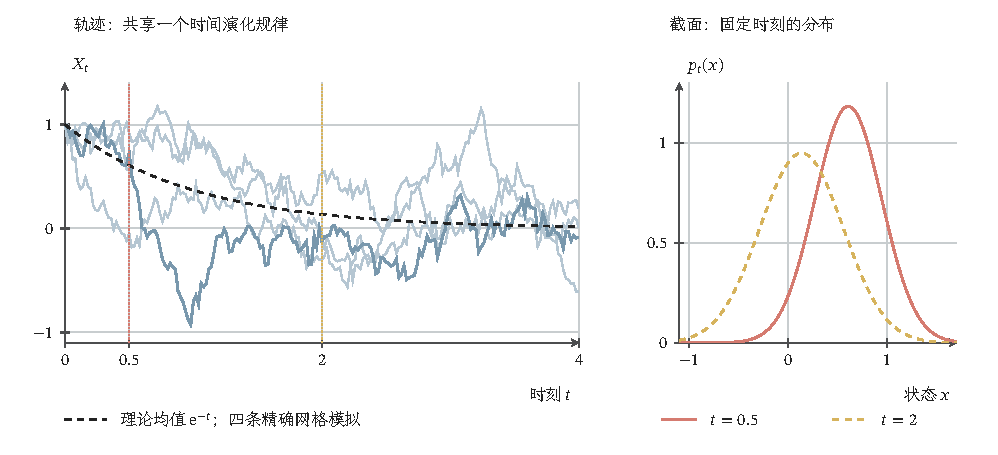
\includegraphics[width=\linewidth]{figures/01-mathematical-preliminaries/05-dynamical-systems-control-decision-and-games/tikz/dynamics/ou-paths-sections.pdf}
 \caption{OU模型的路径与截面。取$\lambda=1,\sigma=0.6,X_0=1$，
 左侧为按精确高斯转移生成的四条网格轨迹与理论均值，右侧为$t=0.5,2$
 的解析边缘密度。折线只连接模拟网格点，不是可微的连续样本路径。
 截面给出单时刻概率，时间间的相关性还由共同噪声与转移决定。}
 \label{fig:action-state-ou-paths}
\end{figure*}

\subsection{随机状态的分布演化}

逐路径的积分式不一定最适合回答“某时刻落在何处”的概率问题。
线性模型可传播少量矩，一般模型则要传播分布对测试函数的作用。
两者都来自同一演化规律，但矩摘要只有在附加分布条件下才是完整描述。

\subsubsection{线性演化下的均值与协方差}

对式~\eqref{eq:action-state-linear-sde-solution}，记
$\bm m_t=\mathbb E\bm X_t,\bm P_t=\operatorname{Cov}(\bm X_t)$。
随机积分为零均值、与初值独立，故
\begin{align*}
 \bm m_t&=\bm\Phi(t,0)\bm m_0+\int_0^t\bm\Phi(t,s)\bm c_s\,\mathrm ds,\\
 \bm P_t&=\bm\Phi(t,0)\bm P_0\bm\Phi(t,0)^\top
       +\int_0^t\bm\Phi(t,s)\bm G_s\bm G_s^\top\bm\Phi(t,s)^\top\,\mathrm ds.
\end{align*}
这里积分中的$\bm G_s\bm G_s^\top$是确定性矩阵。若扩散系数也随机，
就不能直接沿用这组确定性协方差公式；即使均方可积，取期望时也须保留
扩散系数的随机性及其与状态的关系。
两式绝对连续，对几乎处处的$t$有
\begin{align}
 \dot{\bm m}_t&=\bm A_t\bm m_t+\bm c_t,
       \label{eq:dynamical-linear-sde-mean}\\
 \dot{\bm P}_t&=\bm A_t\bm P_t+\bm P_t\bm A_t^\top+\bm G_t\bm G_t^\top.
       \label{eq:dynamical-linear-sde-covariance}
\end{align}
也可令$\widetilde{\bm X}=\bm X-\bm m$，直接用乘积Itô公式得到
\[
 \begin{split}
 \mathrm d(\widetilde{\bm X}\widetilde{\bm X}^{\top})
  ={}&(\bm A\widetilde{\bm X}\widetilde{\bm X}^{\top}
      +\widetilde{\bm X}\widetilde{\bm X}^{\top}\bm A^\top
      +\bm G\bm G^\top)\,\mathrm dt\\
    &+\bm G\,\mathrm d\bm W\,\widetilde{\bm X}^\top
      +\widetilde{\bm X}\,\mathrm d\bm W^\top\bm G^\top .
 \end{split}
\]
二阶矩界使随机积分取期望后消失，得到相同结论。
漂移传播已有不确定性，$\bm G\bm G^\top$持续注入新的不确定性；
后面的离散预测也有同样两项。

OU过程的初值只需平方可积并独立于驱动，就有
\begin{align}
 \mathbb E X_t&=\mathrm e^{-\lambda t}\mathbb E X_0,
       \label{eq:dynamical-ou-mean}\\
 \operatorname{Var}(X_t)&=\mathrm e^{-2\lambda t}\operatorname{Var}(X_0)
       +\frac{\sigma^2}{2\lambda}(1-\mathrm e^{-2\lambda t}).
       \label{eq:dynamical-ou-variance}
\end{align}
均值衰减而方差不消失。对$f(x)=x^2$换元可再次核对：
$\mathrm d(X_t^2)=(-2\lambda X_t^2+\sigma^2)\,\mathrm dt
                 +2\sigma X_t\,\mathrm dW_t$。
若漏掉$\sigma^2\,\mathrm dt$，便会错误地认为持续噪声不留下方差。
当初始分布取$\mathcal N(0,\sigma^2/(2\lambda))$时，OU过程平稳；
一般初态只是在长期趋于该分布，而非每条路径趋于零。
$\sigma=0$时稳态退化为$\delta_0$。非高斯初值的有限时刻分布通常仍非高斯，
上面两个矩不能单独确定它。

\subsubsection{一般演化下的分布与密度}

设确定性系数与适当的解唯一性使$\bm X$成为Markov过程。
要知道分布怎样变化，可先观察任意光滑“读数”$\varphi(\bm X_t)$的短时期望。
\begin{definition}[Itô扩散的生成元]
 \label{def:dynamical-diffusion-generator}
 记$\mathbb E_{t,\bm x}$为从时刻$t$的状态$\bm x$出发的期望。
 对属于算子定义域的测试函数，生成元定义为
 \[
  (\mathcal L_t\varphi)(\bm x)
    =\lim_{h\downarrow0}
       \frac{\mathbb E_{t,\bm x}\varphi(\bm X_{t+h})-\varphi(\bm x)}h.
 \]
 对连续系数的扩散，令$\bm a=\bm\sigma\bm\sigma^\top$；
 在极限与期望可交换时，Itô公式给出
 \[
  \mathcal L_t\varphi=\bm b^\top\nabla\varphi+
                      \tfrac12\operatorname{tr}(\bm a\nabla^2\varphi).
 \]
\end{definition}
从积分Itô公式取条件期望，除以$h$再令$h\downarrow0$，即得最后一式。
例如取光滑紧支撑$\varphi$，并使系数在相关区域有界，可以先局部化来核对该极限。
若时间系数仅可测，则优先使用下面的积分弱式，不强求每个时刻的点态极限。

写$\mu_t$为状态分布。在鞅项可积且均值为零时，
\[
 \int\varphi\,\mathrm d\mu_t-\int\varphi\,\mathrm d\mu_0
     =\int_0^t\int\mathcal L_s\varphi\,\mathrm d\mu_s\,\mathrm ds.
\]
这是不要求密度存在的弱演化式。对有限活动的原计数驱动，还须加上
$\lambda[\varphi(\bm x+\bm\gamma(t,\bm x))-\varphi(\bm x)]$；
若方程用补偿驱动，则漂移算子相应增加
$\lambda[\varphi(\bm x+\bm\gamma)-\varphi(\bm x)
                          -\nabla\varphi^\top\bm\gamma]$。
离散跳跃由有限差算子表达，不是无条件多加一个扩散Hessian项。

若$\mu_t$有密度$p(t,\bm x)$，代入扩散弱式，漂移项分部积分一次，
扩散项分部积分两次，得到
\begin{align*}
 \int\varphi\,\partial_t p\,\mathrm d\bm x
  &=\int\left[\sum_i b_i\partial_i\varphi
            +\tfrac12\sum_{i,j}a_{i,j}\partial_{i,j}\varphi\right]p\,\mathrm d\bm x\\
  &=\int\varphi\left[-\sum_i\partial_i(b_ip)
           +\tfrac12\sum_{i,j}\partial_i\partial_j(a_{i,j}p)\right]\,\mathrm d\bm x .
\end{align*}
测试函数紧支撑时无无穷远边界项；有界区域还需与模型匹配的边界条件。
因此得到\term{Fokker--Planck方程}
\begin{equation}
 \partial_t p=-\sum_i\partial_i(b_ip)
                  +\tfrac12\sum_{i,j}\partial_i\partial_j(a_{i,j}p).
 \label{eq:dynamical-fokker-planck}
\end{equation}
弱等式先成立；经典逐点形式另需$p$和系数的时间、空间正则性。
例如全空间光滑有界系数与一致椭圆扩散是获得正时间光滑密度的一组常用充分条件。
这里一致椭圆（uniformly elliptic）指存在固定$c>0$，使所讨论的时间与状态范围内，
\[
 \bm v^\top\bm a(t,\bm x)\bm v\geq c\|\bm v\|_2^2
 \quad\text{对所有 }\bm v\in\mathbb R^d\text{成立}.
\]
也就是每个方向的噪声强度都有同一个正下界。这比每个$(t,\bm x)$处分别正定更强：后者仍允许最小特征值随状态或时间趋于零。
退化扩散可能把概率留在低维集合，不能预先假定全维光滑密度。

把密度方程写成$\partial_t p=-\nabla\cdot\bm J$，其中
$J_i=b_ip-\frac12\sum_j\partial_j(a_{i,j}p)$。
在$p>0$处，令$\bm v=\bm J/p$，便得到概率流速度
\begin{equation}
 \bm v(t,\bm x)=\bm b(t,\bm x)
   -\tfrac12[\operatorname{div}\bm a(t,\bm x)
                         +\bm a(t,\bm x)\nabla_{\bm x}\log p(t,\bm x)],
 \quad
 (\operatorname{div}\bm a)_i=\sum_j\partial_j a_{i,j}.
 \label{eq:action-state-probability-flow}
\end{equation}
式中的$\bm s_t(\bm x)=\nabla_{\bm x}\log p(t,\bm x)$称为状态密度分数
（state score），表示在状态空间中对数密度上升最快的局部方向。
它对状态$\bm x$求导；前面统计几何中的参数得分对模型参数求导，两者的自变量及向量维数通常不同。
例如OU过程某个时刻的边缘为$\mathcal N(m_t,v_t)$且$v_t>0$时，
$s_t(x)=-(x-m_t)/v_t$，直接指向密度中心，距中心越远时幅度越大。
若此速度的ODE流存在、连续性方程适定，并具有同样初始密度及边界通量，
它便传播同样的边缘密度。只有$\bm a$不依赖状态时，散度项才消失。
流匹配不是路径匹配：ODE在给定初态后无新的噪声，而扩散不断注入随机增量。

时间反演也不是把$b$单独取负。固定终点$T$，用正向反演时钟$s$定义
$\widehat{\bm X}_s=\bm X_{T-s}$。在正密度、系数和密度足够光滑、
扩散非退化及相应可积条件下，其反演滤过中的扩散矩阵为$\bm a(T-s,\bm x)$，
漂移为
\[
 \widehat{\bm b}(s,\bm x)
    =-\bm b(T-s,\bm x)+\operatorname{div}\bm a(T-s,\bm x)
                  +\bm a(T-s,\bm x)\nabla_{\bm x}\log p(T-s,\bm x).
\]
例如可先在远离奇异端点的紧时间区间上取光滑有界系数、一致椭圆矩阵、
正的光滑密度及局部可积的分数，并另保证反演方程无爆炸。
反演Brownian运动相对于反演历史定义，不能当作原Brownian路径简单反号。
这一结果还用到正反向转移的Bayes关系；前向密度方程本身不确定时间间联合规律。
在生成模型中用估计分数替换真实分数，会再引入模型误差。

\subsection{随机轨迹的模拟与采样}

有限时域模拟问数值状态是否接近给定随机模型；长期采样问所构造的链是否按目标
分布取样。前一问题可以比较耦合路径或测试函数，后一问题还要检查不变性、遍历性
和混合速度。两者都使用随机数，但保证的对象不同。

\subsubsection{有限时域的轨迹模拟}

固定$T$，取$t_k=kh$、$n=T/h$为整数，初值
$\widehat{\bm X}_0=\bm X_0$。Euler--Maruyama方法冻结每段左端的系数：
\begin{equation}
 \widehat{\bm X}_{k+1}=\widehat{\bm X}_k+
    h\bm b(t_k,\widehat{\bm X}_k)
    +\bm\sigma(t_k,\widehat{\bm X}_k)\sqrt h\,\bm\varepsilon_k,
 \qquad \bm\varepsilon_k\overset{\mathrm{iid}}{\sim}\mathcal N(\bm0,\bm I_m).
 \label{eq:dynamical-euler-maruyama}
\end{equation}
新噪声与初值、先前噪声独立。扩散项乘$\sqrt h$，才能每单位时间累计有限方差；
随机逼近中的步长乘观测误差通常是$h\xi_k$，方差尺度为$h^2$，两者不是同一极限。

Poisson驱动须另生成$\Delta N_k\sim\operatorname{Pois}(\lambda h)$，
并按驱动假设与Brownian增量独立。网格法用
$\bm\gamma(t_k,\widehat{\bm X}_k)\Delta N_k$冻结该段跳幅；
补偿版本改用$\Delta N_k-\lambda h$。当一段内有多个事件且跳幅依赖状态时，
这种冻结不同于逐事件更新。
事件适配法则依次采样独立$\operatorname{Exp}(\lambda)$等待时间，
把跳时插入网格，在事件间模拟扩散、在事件处用跳前状态更新。
这里Brownian增量仍按各段实际长度采样，不能用高斯增量冒充跳跃计数。

\paragraph{同一噪声下的状态误差}

强误差必须把算法和真解放在同一个驱动上，即令
$\sqrt h\,\bm\varepsilon_k=\bm W_{t_{k+1}}-\bm W_{t_k}$。
对自治系数，在全局Lipschitz、线性增长和$\bm X_0\in L^2$条件下，
固定有限时域有
\[
 \max_{0\leq k\leq n}
   \bigl(\mathbb E\|\bm X_{t_k}-\widehat{\bm X}_k\|^2\bigr)^{1/2}
     \leq C_T h^{1/2}.
\]
显式时间依赖时，一组充分条件是统一状态Lipschitz，并有
$\|\bm b(t,\bm x)-\bm b(s,\bm x)\|
 +\|\bm\sigma(t,\bm x)-\bm\sigma(s,\bm x)\|_{\mathrm F}
 \leq K(1+\|\bm x\|)|t-s|^{1/2}$。
常数依赖$T$和系数界，不是无限时域的统一保证。

估计机制与存在性证明相连。定义连续插值
\[
 \begin{split}
 \widehat{\bm X}_t={}&\bm X_0+
    \int_0^t\bm b(\eta(s),\widehat{\bm X}_{\eta(s)})\,\mathrm ds\\
 &+\int_0^t\bm\sigma(\eta(s),\widehat{\bm X}_{\eta(s)})\,\mathrm d\bm W_s,
 \end{split}
\]
其中$\eta(s)=t_{\lfloor s/h\rfloor}$，插值在网格上等于算法值。
增长界先给出统一二阶矩，并由等距得到
$\sup_{s\leq T}\mathbb E\|\widehat{\bm X}_s-\widehat{\bm X}_{\eta(s)}\|^2
\leq C_T h$。相减积分方程，用Lipschitz、最大不等式和时间正则性得
\[
 E(t):=\mathbb E\sup_{r\leq t}\|\bm X_r-\widehat{\bm X}_r\|^2
       \leq C_T\int_0^tE(s)\,\mathrm ds+C_T h.
\]
Grönwall给出$E(T)\leq C'_T h$，开方即得强半阶。
加性噪声等结构可能提高阶数，但不是一般乘性噪声的保证；
跳跃扩展还需另核对跳幅、驱动耦合与事件处理。

\paragraph{测试函数下的期望误差}

弱误差不逐路径相减，而是比较读数的期望。一组方便的自治充分条件是漂移、
扩散与测试函数$\varphi$具有至四阶连续有界导数，并满足增长和所需矩条件；
更保守地可取它们本身及至四阶导数均有界。此时
\[
  |\mathbb E\varphi(\bm X_T)-\mathbb E\varphi(\widehat{\bm X}_n)|
        \leq C_{\varphi,T}h.
\]
其机制是对剩余期望函数
$u(t,\bm x)=\mathbb E_{t,\bm x}\varphi(\bm X_T)$作局部展开。
在其相应导数有界的条件下，精确转移与一次Euler转移都给出
$u+h\mathcal L u+O(h^2)$。把每步的期望差望远镜相加，
$n=T/h$个局部$O(h^2)$误差累计为$O(h)$。
这里引用标准弱收敛结果，导数与矩条件用于保证展开余项统一可积；
不能仅凭二阶矩和状态Lipschitz就断言弱一阶。\scite{math-kloeden1992numerical-sde}

弱阶较高不说明两条样本轨迹更接近。例如独立生成的两个同分布终点对所有可积
测试函数期望完全相同，彼此状态距离却不为零。有限时间弱误差还不能直接交换
$h\downarrow0$与$T\uparrow\infty$，长期步长偏差必须单独分析。

\subsubsection{目标分布下的长期采样}

设目标密度$\pi>0$光滑且可归一化。过阻尼Langevin模型为
\begin{equation}
 \mathrm d\bm X_t=\tfrac12\nabla\log\pi(\bm X_t)\,\mathrm dt+\mathrm d\bm W_t.
 \label{eq:dynamical-langevin-sde}
\end{equation}
代入Fokker--Planck通量，$\bm b\pi-\nabla\pi/2=\bm0$。
在方程无爆炸、边界通量为零及密度方程适定等条件下，这证明$\pi$不变。
从其他初态收敛还需遍历条件；例如$\pi\propto\mathrm e^{-U}$，
$U$光滑强凸且梯度全局Lipschitz时，噪声非退化与向内漂移提供常用保证。
多峰势能可能保持同一目标却混合很慢。

即使连续模型正确，离散化也会改变稳态。取$\pi=\mathcal N(0,1)$，
则$X_{k+1}=(1-h/2)X_k+\sqrt h\,\varepsilon_k$。
只有$0<h<4$时这一递推稳定，其稳态方差为
\[
  \frac{h}{1-(1-h/2)^2}=\frac1{1-h/4},
\]
并非$1$。减小步长减小偏差，但在相同计算步数下也缩短模拟时间；
有限预算须同时考虑初态遗留、相关性和离散误差。

Hamilton蒙特卡洛（HMC）使用另一种构造。若
$\pi(\bm q)\propto\exp[-U(\bm q)]$，引入独立
$\bm p\sim\mathcal N(\bm0,\bm M)$，联合密度为
$\rho(\bm q,\bm p)\propto\exp[-H(\bm q,\bm p)]$。
精确Hamilton流保持能量和体积，因此保持$\rho$；
蛙跳只保持体积与可逆结构，需要接受校正补偿能量误差。
固定步长$h$与步数$L$，记$T=R\circ\Psi_h^L$，
其中$R(\bm q,\bm p)=(\bm q,-\bm p)$。
前面已证明$R\Psi_hR=\Psi_h^{-1}$，故$T^2=I$，且$|\det DT|=1$。
对$\bm z' =T\bm z$，接受概率取
\begin{equation}
 \alpha(\bm z)=\min\{1,\exp[-H(\bm z')+H(\bm z)]\}.
 \label{eq:dynamical-hmc-acceptance}
\end{equation}

\begin{theorem}[HMC提议的详细平衡]
 \label{thm:action-state-hmc-balance}
 若$T$是可微、体积保持的对合，则以概率$\alpha(\bm z)$移至$T\bm z$，
 否则留在$\bm z$的核，对密度$\rho$满足详细平衡。
\end{theorem}
\begin{proof}
 接受部分的密度权重为
 $\rho(\bm z)\alpha(\bm z)=\min\{\rho(\bm z),\rho(T\bm z)\}$。
 对任意有界可测函数$g(\bm z,\bm z')$，作变量替换$\bm y=T\bm z$，
 由$T^2=I$和单位绝对Jacobian，
 \[
 \begin{split}
 &\int g(\bm z,T\bm z)\min\{\rho(\bm z),\rho(T\bm z)\}\,\mathrm d\bm z\\
 &\quad=\int g(T\bm y,\bm y)
                   \min\{\rho(T\bm y),\rho(\bm y)\}\,\mathrm d\bm y .
 \end{split}
 \]
 这证明接受部分在交换出发与到达状态后不变。
 拒绝部分集中在对角线$\bm z'=\bm z$，本身对称，两者相加即为详细平衡。
\end{proof}

一轮算法因而是：保留当前位置并重新抽取高斯动量；按三子步蛙跳执行$L$次；
翻转末端动量并计算$\Delta H$；抽取独立均匀数，按
$\min(1,\mathrm e^{-\Delta H})$接受，否则保留原位置。
动量刷新是联合目标的条件抽样，保持$\rho$；再接上述核仍保持$\rho$，
边缘化动量得到位置目标$\pi$。两个保持核的复合不必在联合空间仍可逆，
此处不把复合的不变性误说成自动详细平衡。

若提议不保持体积，接受比还需Jacobian因子；状态依赖地改变步数或步长，
也须重新核对反向提议。实现中的有限精度可逆误差不是上述精确算术证明的一部分。
接受校正不保证独立样本或快速混合：步长过大导致拒绝，轨迹过短导致高相关，
质量矩阵失配使不同方向移动不均衡。采样以保持分布为目标，不要求能量一路下降，
所以不能将Hamilton轨迹解释为更快的梯度下降。

\begin{table*}[htbp]
 \centering
 \begin{tabularx}{\linewidth}{lXX}
 \toprule
 结论 & 所比较的对象 & 尚未得到的保证\\
 \midrule
 强数值误差小 & 同一驱动下数值状态与真状态 & 长期抽样偏差小\\
 弱数值误差小 & 两种状态分布的测试函数期望 & 单条路径距离小\\
 密度$\pi$不变 & 从$\pi$出发仍保持$\pi$ & 其他初态快速趋于$\pi$\\
 概率流匹配边缘 & 每个时刻的状态分布 & 相同时间间联合规律\\
 \bottomrule
 \end{tabularx}
 \caption{随机演化中几种保证的对象。每一项均依赖当地给出的正则、边界或数值条件，
 不能用一个对象上的结论替代另一个对象上的结论。}
 \label{tab:dynamical-path-distribution}
\end{table*}

\section{随机状态的观测与推断}
\label{sec:dynamical-state-space-filtering}
\label{sec:dynamical-stochastic-state-observation}

过程噪声规定真实状态如何随机移动；传感器读数则提供关于这条未知轨迹的证据。
因此推断不是再次生成一条任意轨迹，而是在已给定的生成模型中，保留与读数相容的
状态并重新分配概率。先明确可见数据与查询目标，再把预测、滤波和平滑化为可计算公式。

\subsection{状态观测与推断目标}

在前面的状态转移$K_t$之外增加观测核
$G_t(\bm x,B)=\mathbb P(\bm y_t\in B\mid\bm x_t=\bm x)$。
它表示状态为$\bm x$时传感器返回哪些读数。线性加性例为
\begin{equation}
  \bm y_t=\bm C_t\bm x_t+\bm v_t.
  \label{eq:dynamical-linear-observation-model}
\end{equation}
先假设初值、所有过程噪声与所有观测噪声相互独立，输入与矩阵给定。
于是给定$\bm x_t$后，$\bm y_t$不再依赖旧状态和旧观测；
给定当前状态后，下一状态由$K_t$生成。联合规律在
式~\eqref{eq:dynamical-linear-state-model}的基础上分解为
\[
 \pi_0(\mathrm d\bm x_0)
       \prod_{t=0}^{T-1}K_t(\bm x_t,\mathrm d\bm x_{t+1})
       \prod_{t=1}^T G_t(\bm x_t,\mathrm d\bm y_t).
\]
这里从$y_1$开始观察，$\pi_0$不含一个未声明的$y_0$。
若噪声相关、传感器依赖旧状态或有内部滞后，须扩充联合状态或显式改写这些
条件关系。观测序列通常不满足自身的Markov性，因为一次带噪读数未必概括隐藏状态。

记$\mathcal Y_t=\sigma(\bm y_1,\ldots,\bm y_t)$，
$\mathcal Y_0$为无观测信息。欧氏状态与观测具有正则条件分布，
使“给定这段读数的状态概率”能作为概率核处理。
即使观测无噪，也不一定足够：$y_t=x_{1,t}+x_{2,t}$不能区分
$(1,0)^\top$与$(0,1)^\top$。能否借后续动力学区分这些方向，需要
第~\ref{chap:control-theory}章的可观测性与可检测性条件。

\begin{example}[带泄漏温度的间接观测]
 \label{ex:dynamical-noisy-temperature}
 回到同一模型
 $x_{t+1}=0.8x_t+u_t+w_{t+1}$、$y_t=x_t+v_t$，
 其中$w_t\sim\mathcal N(0,0.04)$、$v_t\sim\mathcal N(0,0.09)$，
 与初值及彼此独立。即使传感器完全精确，未来仍因$w_{t+1}$不确定；
 即使过程无噪，当前状态也可能因读数噪声而不确定。
 图~\ref{fig:action-state-temperature-layers}的轨迹从已知$x_0=0$出发，
 使用给定$u_t=0.4$；后面的估计继续使用该初值与同一组读数，
 不另换一条更利于展示的状态轨迹。
\end{example}

得到条件分布后，还须规定输出什么估计。平方损失下，若$\bm X$二阶可积，
对信息$\mathcal G$可测的估计$\bm a$，
\[
 \mathbb E[\|\bm X-\bm a\|^2\mid\mathcal G]
 =\mathbb E[\|\bm X-\mathbb E(\bm X\mid\mathcal G)\|^2\mid\mathcal G]
       +\|\mathbb E(\bm X\mid\mathcal G)-\bm a\|^2.
\]
交叉项因条件均值为零而消失，所以条件均值最小化均方损失。
离散状态的零一损失选条件众数；连续密度的MAP是另一种点输出，
不能不说明损失就把所有“最优估计”视为同义。

\subsection{不同观测范围下的边缘状态推断}
\label{sec:dynamical-kalman-rts}

固定目标时刻$t$，改变可用观测的终点$j$。记
$\bm m_{t\mid j}=\mathbb E[\bm x_t\mid\mathcal Y_j]$、
$\bm P_{t\mid j}=\operatorname{Cov}(\bm x_t\mid\mathcal Y_j)$。
三种查询的区别先由信息范围决定，与使用哪一种算法无关。

\begin{table}[htbp]
 \centering
 \begin{tabularx}{\linewidth}{lXX}
 \toprule
 查询 & 目标条件分布 & 允许的观测\\
 \midrule
 一步预测 & $P(\bm x_t\mid\mathcal Y_{t-1})$ & 新读数以前\\
 当前滤波 & $P(\bm x_t\mid\mathcal Y_t)$ & 包括当前读数\\
 固定区间平滑 & $P(\bm x_t\mid\mathcal Y_T)$，$T>t$ & 包括事后未来读数\\
 \bottomrule
 \end{tabularx}
 \caption{同一目标状态的三种边缘查询。信息终点改变，物理状态并未改变；
 平滑使用的未来读数不能用于当时的在线行动。}
 \label{tab:dynamical-estimation-information}
\end{table}

下面的一般核公式只要求前述条件独立结构。需要解析闭合时，再采用有限时域
线性高斯条件：
\[
 \bm x_0\sim\mathcal N(\bm m_{0\mid0},\bm P_{0\mid0}),\quad
 \bm w_{t+1}\sim\mathcal N(\bm0,\bm Q_{t+1}),\quad
 \bm v_t\sim\mathcal N(\bm0,\bm R_t).
\]
三组随机量彼此独立，系统矩阵与输入确定，
$\bm P_{0\mid0},\bm Q_{t+1}\succeq\bm0$，先取$\bm R_t\succ\bm0$。
本章统一让$w_{t+1}$与它推动到达的状态时刻一致；
因此从$t-1$到$t$的过程协方差写为$\bm Q_t$。
这些条件在每个有限$T$内使用，不预设滤波增益已达稳态。

\subsubsection{过去观测下的状态预测}

若已有截至$t-1$的条件分布$\pi_{t-1}$，全概率公式给出
\begin{equation}
 \pi_{t\mid t-1}(A)
     =\int K_{t-1}(\bm x,A)\,\pi_{t-1}(\mathrm d\bm x).
 \label{eq:dynamical-general-prediction-kernel}
\end{equation}
这是把每个候选旧状态的下一步分布，按其当前可信程度混合。
多步预测重复施加转移核，中途没有新观测便没有似然校正。

例如隐藏状态为$\{0,1\}$，$\pi_0=(0.7,0.3)$，
按当前状态为行、下一状态为列的转移矩阵为
$\bm P=\left[\begin{smallmatrix}0.8&0.2\\0.1&0.9\end{smallmatrix}\right]$。
于是$\pi_{1\mid0}(1)=0.7(0.2)+0.3(0.9)=0.41$，
$\pi_{1\mid0}(0)=0.59$。这是尚未看$y_1$的结果；
下一小节再用同一预测做校正。

在线性高斯条件下，仿射变换与独立高斯相加保持高斯性，所以
\begin{align}
 \bm m_{t\mid t-1}
   &=\bm A_{t-1}\bm m_{t-1\mid t-1}+\bm B_{t-1}\bm u_{t-1},
       \label{eq:dynamical-kalman-predicted-mean}\\
 \bm P_{t\mid t-1}
   &=\bm A_{t-1}\bm P_{t-1\mid t-1}\bm A_{t-1}^\top+\bm Q_t.
       \label{eq:dynamical-kalman-predicted-covariance}
\end{align}
温度第一步为$m_{1\mid0}=0.4,P_{1\mid0}=0.04$：
初值已知并不等于未来状态已知。一般预测方差并非必然大于旧方差，
因为$\bm A$可能收缩；过程噪声是在已传播的协方差之上增加$\bm Q_t$。
若$w_t$与旧状态相关，须增加
$\bm A_{t-1}\operatorname{Cov}(\bm x_{t-1},\bm w_t\mid\mathcal Y_{t-1})$
及其转置，并使用噪声的条件均值和条件协方差。
未经核对独立性就删交叉项，会改变预测。

\subsubsection{当前及过去观测下的状态滤波}

\begin{definition}[滤波分布]
 \label{def:dynamical-filtering-distribution}
 当前状态在截至当前的观测信息下的条件概率核
 \begin{equation}
  \pi_t(A)=\mathbb P(\bm x_t\in A\mid\mathcal Y_t)
   \label{eq:dynamical-filtering-distribution}
 \end{equation}
 称为\term{滤波分布}。它与真实状态$\bm x_t$、实际读数$\bm y_t$分别是
 推断结果、潜在对象与数据。
\end{definition}

若观测核有相对于共同$\sigma$有限测度$\nu_t$的联合可测密度
$G_t(\bm x,\mathrm d\bm y)=g_t(\bm y\mid\bm x)\nu_t(\mathrm d\bm y)$，
则Bayes公式给出
\begin{equation}
 \pi_t(\mathrm d\bm x)=
 \frac{g_t(\bm y_t\mid\bm x)\pi_{t\mid t-1}(\mathrm d\bm x)}
      {\int g_t(\bm y_t\mid\bm z)\pi_{t\mid t-1}(\mathrm d\bm z)}.
 \label{eq:dynamical-general-bayes-filter}
\end{equation}
分母必须有限且严格为正。共同支配测度不依赖候选状态，才能把这些似然放在同一
尺度比较；没有这种密度表示时仍有正则条件分布，但不能生搬该比值。

\begin{example}[两状态模型的一次预测与校正]
 \label{ex:dynamical-two-state-bayes-filter}
 接续上一小节的预测结果。若
 $\mathbb P(y_1=1\mid x_1=0)=0.2$、
 $\mathbb P(y_1=1\mid x_1=1)=0.8$，实际看到$y_1=1$后，
 \[
  \pi_1(1)=\frac{0.8(0.41)}{0.2(0.59)+0.8(0.41)}
              =\frac{164}{223}\approx0.735.
 \]
 新证据使状态$1$的相对权重上升。只需$\pi_0$而不重新读取更早观测，
 是因为条件独立结构已经把过去对未来有用的信息压入该分布。
\end{example}

在线性高斯模型中，上面的密度乘积可以用一次联合高斯条件化完成。
给定$\mathcal Y_{t-1}$，
\begin{equation}
 \begin{bmatrix}\bm x_t\\\bm y_t\end{bmatrix}
 \sim\mathcal N\left(
 \begin{bmatrix}\bm m_{t\mid t-1}\\\bm C_t\bm m_{t\mid t-1}\end{bmatrix},
 \begin{bmatrix}
  \bm P_{t\mid t-1}&\bm P_{t\mid t-1}\bm C_t^\top\\
  \bm C_t\bm P_{t\mid t-1}&\bm S_t
 \end{bmatrix}\right),
 \label{eq:dynamical-kalman-joint-gaussian}
\end{equation}
其中\term{创新协方差}为
\begin{equation}
 \bm S_t=\bm C_t\bm P_{t\mid t-1}\bm C_t^\top+\bm R_t.
 \label{eq:dynamical-kalman-innovation-covariance}
\end{equation}
创新$\bm r_t=\bm y_t-\bm C_t\bm m_{t\mid t-1}$是读数超出预测观测的部分。
$\bm R_t\succ\bm0$保证$\bm S_t$可逆。由条件高斯公式，
\begin{align}
 \bm K_t&=\bm P_{t\mid t-1}\bm C_t^\top\bm S_t^{-1},
       \label{eq:dynamical-kalman-gain}\\
 \bm m_{t\mid t}&=\bm m_{t\mid t-1}+\bm K_t\bm r_t,
       \label{eq:dynamical-kalman-filtered-mean}\\
 \bm P_{t\mid t}&=\bm P_{t\mid t-1}-\bm K_t\bm S_t\bm K_t^\top.
       \label{eq:dynamical-kalman-filtered-covariance}
\end{align}
Kalman增益$\bm K_t$由两类误差协方差决定，不是自由设置的学习率。
减去的是半正定项，所以这次高斯校正不增加条件协方差。
一般非高斯模型中，“更多信息减少均方误差”是平均意义的结论，
不保证每个罕见读数对应的后验方差都比先验小。\scite{math-kalman1960filtering}

\begin{theorem}[有限时域Kalman滤波]
 \label{thm:dynamical-finite-horizon-kalman-filter}
 在上述独立线性高斯模型与创新协方差可逆条件下，预测与校正公式精确给出
 $\bm x_t\mid\mathcal Y_t\sim
       \mathcal N(\bm m_{t\mid t},\bm P_{t\mid t})$，对每个有限$t$成立。
\end{theorem}
\begin{proof}
 $t=0$时无观测，条件分布就是给定高斯初值。假设上一时刻结论成立，
 独立高斯过程噪声与线性状态更新得到式
 ~\eqref{eq:dynamical-kalman-predicted-mean}和
 ~\eqref{eq:dynamical-kalman-predicted-covariance}，并保持高斯性。
 独立高斯观测噪声又给出式~\eqref{eq:dynamical-kalman-joint-gaussian}。
 为核对条件化，令$\bm e=\bm x_t-\bm m_{t\mid t-1}-\bm K_t\bm r_t$。
 在$\mathcal Y_{t-1}$条件下，
 $\operatorname{Cov}(\bm e,\bm r_t)
   =\bm P_{t\mid t-1}\bm C_t^\top-\bm K_t\bm S_t=\bm0$。
 联合高斯中不相关即独立，所以给定新读数后$\bm e$仍为零均值高斯，
 协方差为$\bm P_{t\mid t-1}-\bm K_t\bm S_t\bm K_t^\top$。
 新条件均值与协方差正是上述校正式，归纳完成。
\end{proof}

把估计误差写成
$(\bm I-\bm K_t\bm C_t)(\bm x_t-\bm m_{t\mid t-1})-\bm K_t\bm v_t$，
利用两项误差独立，得到Joseph形式
\begin{equation}
 \bm P_{t\mid t}=(\bm I-\bm K_t\bm C_t)\bm P_{t\mid t-1}
                    (\bm I-\bm K_t\bm C_t)^\top+\bm K_t\bm R_t\bm K_t^\top.
 \label{eq:dynamical-kalman-joseph-form}
\end{equation}
展开并用$\bm K_t\bm S_t=\bm P_{t\mid t-1}\bm C_t^\top$，
即恢复简化校正式。半正定项相加的形式更利于有限精度下维持协方差性质；
实现应解线性方程求增益作用，不显式形成$\bm S_t^{-1}$。

\begin{example}[标量观测怎样权衡预测与读数]
 \label{ex:dynamical-scalar-kalman-update}
 对$y=x+v$、$v\sim\mathcal N(0,r)$，有
 $K=p^-/(p^-+r)$、$m^+=m^-+K(y-m^-)$、$p^+=p^-r/(p^-+r)$。
 独立任务例取$(m^-,p^-,r,y)=(0,4,1,2)$，得到
 $K=4/5,m^+=8/5,p^+=4/5$。
 温度模型则仍用$r=0.09$，第一步增益为$0.04/0.13=4/13$，
 $m_{1\mid1}=0.4+\frac4{13}(y_1-0.4)$、
 $P_{1\mid1}=0.036/1.3\approx0.02769$。
 两例用于比较同一公式，不能互换噪声参数。
\end{example}

观测越精确，直接观测方向的增益通常越大；未被$\bm C_t$区分的方向可能仍有
不确定性。图~\ref{fig:dynamical-kalman-density-update}显示标量分布如何重加权：
密度变高表示质量集中，不是单点概率大于$1$。
\begin{figure}[htbp]
 \centering
 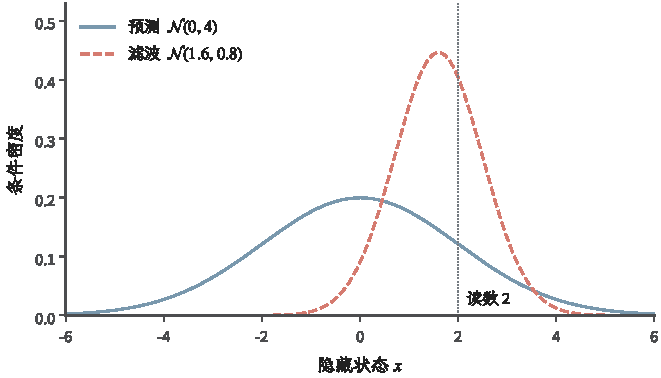
\includegraphics[width=\linewidth]{figures/01-mathematical-preliminaries/05-dynamical-systems-control-decision-and-games/matplotlib/dynamics/kalman-density-update.pdf}
 \caption{独立标量教学例的预测$\mathcal N(0,4)$与后验$\mathcal N(1.6,0.8)$，
 实际读数$y=2$、观测噪声方差$1$。第二个高斯参数是方差；
 本图不是贯穿温度模型的参数设定。}
 \label{fig:dynamical-kalman-density-update}
\end{figure}
\FloatBarrier

若状态更新为$\bm x_{t+1}=\bm f_t(\bm x_t)+\bm w_{t+1}$，
观测为$\bm y_t=\bm h_t(\bm x_t)+\bm v_t$，查询仍是同一个滤波分布，
只是高斯闭合一般失效。扩展Kalman滤波（EKF）在滤波均值附近以
$\bm F_t=D\bm f_t(\bm m_{t\mid t})$传播协方差，
预测均值取$\bm f_t(\bm m_{t\mid t})$；
在预测均值处以$\bm H_{t+1}=D\bm h_{t+1}(\bm m_{t+1\mid t})$
构造创新协方差和增益。它把局部函数替换为一阶线性函数，
所以通常既忽略曲率对均值的影响，也把后验压回单个高斯。

无迹Kalman滤波（UKF）用确定性sigma点近似非线性矩传播。
例如对$d$维均值$\bm m$与协方差$\bm P=\bm L\bm L^\top$，
取$\kappa\geq0$，点为$\bm m$及
$\bm m\pm\sqrt{d+\kappa}\bm L_{\cdot i}$，权重分别为
$\kappa/(d+\kappa)$与$1/[2(d+\kappa)]$。
它们精确匹配原均值与协方差。将点代入$\bm f$，以加权和、加权外积估计
新均值与协方差，再给协方差加上过程噪声$\bm Q$。
本处采用重新生成点的实现：依据加入$\bm Q$后的预测均值和协方差重新构造sigma点，
再把这组点送入$\bm h$，计算预测观测均值、观测协方差及状态观测交叉协方差。
观测协方差还须加上观测噪声$\bm R$，随后按Kalman的创新与增益公式校正。
重新生成点使观测预测也包含本步新增的过程不确定性。
例如标量线性系统$f(x)=h(x)=x$，旧状态方差$p=1$，过程与观测噪声方差
$q=r=1$，上述步骤给出预测方差$2$、创新方差$3$、交叉方差$2$，故增益为$2/3$，
与精确Kalman公式一致；直接复用未包含$q$的原传播点则无法得到这个结果。
这是简单的非负权重构造，实际UKF还可使用带缩放参数的不同权重。
其近似发生在矩积分和高斯投影，不是把非线性模型变成精确线性模型。

两种方法都可能遗漏多峰后验。例如零均值对称先验配上
$y=x^2+v$，一个明显正的读数可能支持正负两个状态区间。
EKF在$x=0$的观测导数为零；对称sigma点也有零状态观测交叉协方差，
单高斯校正不能表达分裂成两峰的证据。
粒子滤波改用加权经验分布$\sum_i\omega_t^{(i)}\delta_{x_t^{(i)}}$：
从已有粒子按转移核抽下一状态，将权重乘当前似然再归一化，
必要时按权重重采样。其近似对象是整个滤波概率测度，
并用有限样本替代核积分；权重集中、高维与重采样损失多样性仍是限制。
高斯混合则保留多个分量，分别传播和校正，再用似然更新分量权重；
分量合并或剪枝会引入另一种近似。

\subsubsection{有限时域完整观测下的状态平滑}

固定终点$T$后，未来读数也能帮助判断旧状态。关键不是再向前预测，
而是把新获得的下一状态分布通过反向条件关系传回去。
在线性高斯条件下，给定$\mathcal Y_t$，
\[
 \begin{bmatrix}\bm x_t\\\bm x_{t+1}\end{bmatrix}
 \sim\mathcal N\left(
 \begin{bmatrix}\bm m_{t\mid t}\\\bm m_{t+1\mid t}\end{bmatrix},
 \begin{bmatrix}
  \bm P_{t\mid t}&\bm P_{t\mid t}\bm A_t^\top\\
  \bm A_t\bm P_{t\mid t}&\bm P_{t+1\mid t}
 \end{bmatrix}\right).
\]
若$\bm P_{t+1\mid t}$可逆，条件高斯公式给出
\begin{align}
 \bm J_t&=\bm P_{t\mid t}\bm A_t^\top\bm P_{t+1\mid t}^{-1},
    \label{eq:dynamical-rts-gain}\\
 \mathbb E[\bm x_t\mid\bm x_{t+1},\mathcal Y_t]
   &=\bm m_{t\mid t}+\bm J_t(\bm x_{t+1}-\bm m_{t+1\mid t}),
    \label{eq:dynamical-rts-one-step-conditional-mean}\\
 \operatorname{Cov}(\bm x_t\mid\bm x_{t+1},\mathcal Y_t)
   &=\bm P_{t\mid t}-\bm J_t\bm P_{t+1\mid t}\bm J_t^\top.
    \label{eq:dynamical-rts-one-step-conditional-covariance}
\end{align}
这里的$\bm J_t$关联相邻状态，不是由当前传感器直接得到的Kalman增益。

\begin{theorem}[有限时域RTS平滑]
 \label{thm:dynamical-rts-smoother}
 在有限时域Kalman条件及每个$\bm P_{t+1\mid t}$可逆条件下，
 从终点$(\bm m_{T\mid T},\bm P_{T\mid T})$向后递推
 \begin{align}
  \bm m_{t\mid T}
   &=\bm m_{t\mid t}+\bm J_t(\bm m_{t+1\mid T}-\bm m_{t+1\mid t}),
       \label{eq:dynamical-rts-smoothed-mean}\\
  \bm P_{t\mid T}
   &=\bm P_{t\mid t}
         +\bm J_t(\bm P_{t+1\mid T}-\bm P_{t+1\mid t})\bm J_t^\top,
       \label{eq:dynamical-rts-smoothed-covariance}
 \end{align}
 精确给出$\bm x_t\mid\mathcal Y_T$的高斯均值与协方差。
\end{theorem}
\begin{proof}
 给定$\bm x_{t+1}$后，未来状态和观测与更早状态条件独立，因此
 $P(\mathrm d\bm x_t\mid\bm x_{t+1},\mathcal Y_T)
   =P(\mathrm d\bm x_t\mid\bm x_{t+1},\mathcal Y_t)$。
 全概率公式给出后向因子化
 \begin{equation}
  P(\mathrm d\bm x_t\mid\mathcal Y_T)
   =\int P(\mathrm d\bm x_t\mid\bm x_{t+1},\mathcal Y_t)
                   P(\mathrm d\bm x_{t+1}\mid\mathcal Y_T).
  \label{eq:dynamical-rts-backward-factorization}
 \end{equation}
 将一步条件均值对$\bm x_{t+1}\mid\mathcal Y_T$取期望，
 塔式性质得到平滑均值公式。全协方差公式分成两项：条件内协方差为
 $\bm P_{t\mid t}-\bm J_t\bm P_{t+1\mid t}\bm J_t^\top$，
 条件均值的协方差为$\bm J_t\bm P_{t+1\mid T}\bm J_t^\top$；
 相加即得平滑协方差。一步条件核的均值为仿射函数、协方差不依赖下一状态，
 与高斯下一状态混合仍为高斯。从$T$向后归纳，完成全部时刻的结论。
\end{proof}

前向保存每步滤波与预测的均值、协方差，后向依次计算$\bm J_t$及上述两式，
就是Rauch--Tung--Striebel（RTS）平滑算法。\scite{math-rauch1965smoothing}
未来观测影响过去的条件分布，不改变已经发生的物理状态。

\begin{example}[未来观测降低过去状态的不确定性]
 \label{ex:dynamical-scalar-rts-update}
 用独立随机游走例$x_1=x_0+w_1$、$y_1=x_1+v_1$，
 取$m_{0\mid0}=0,P_{0\mid0}=1,Q_1=1,R_1=2/3$且噪声独立。
 观察$y_1=2$后，$m_{1\mid0}=0,P_{1\mid0}=2$，
 $K_1=3/4,m_{1\mid1}=3/2,P_{1\mid1}=1/2$。
 于是$J_0=1/2$，$m_{0\mid1}=3/4$，
 $P_{0\mid1}=1+\frac14(\frac12-2)=5/8$。
 在时刻$0$尚不能使用这个结果；此时只有均值$0$、方差$1$的初始先验。
\end{example}

\begin{figure*}[htbp]
 \centering
 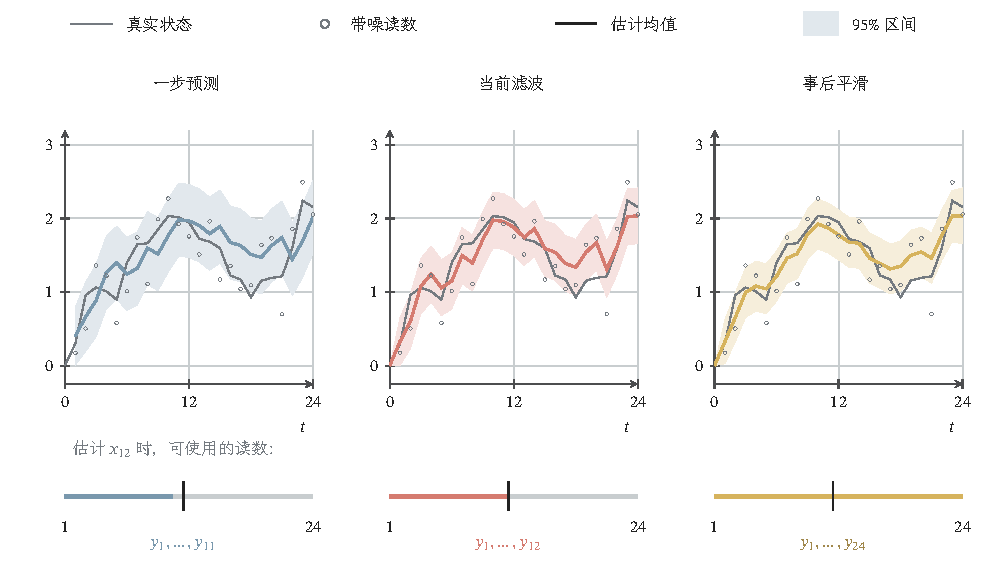
\includegraphics[width=\linewidth]{figures/01-mathematical-preliminaries/05-dynamical-systems-control-decision-and-games/tikz/dynamics/temperature-inference.pdf}
 \caption{与图~\ref{fig:action-state-temperature-layers}完全相同的温度轨迹及读数。
 三栏分别画一步预测、滤波与固定终点$T=24$的平滑均值和逐时刻$95\%$高斯区间，
 灰线为实际状态，圆点为读数；区间不是整条路径同时覆盖的置信带。
 下方以$t=12$为例标出可用观测范围。已知$x_0=0$，给定$u_t=0.4$，
 过程、观测方差仍为$0.04,0.09$。平滑的信息优势不是额外的在线能力。}
 \label{fig:action-state-temperature-inference}
\end{figure*}

图中的高斯平滑协方差不超过相应滤波协方差，但某一条实现上的均值误差不必
每个时刻都更小。条件均方误差的保证与某一次噪声实现上的误差是不同对象。
若预测协方差奇异，须在其仿射支持上条件化，广义逆只是计算工具，
还要检查条件状态是否属于支持，不能只替换逆号。
非线性近似平滑可沿相同后向关系用局部线性化或sigma点估计相邻状态的交叉矩；
粒子平滑则近似反向核或路径权重。无论采用哪种表示，使用$\mathcal Y_T$
这一信息条件都不改变。

\subsection{完整观测下的联合轨迹推断}

各时刻边缘分布回答“那一刻可能在哪里”，整条路径后验还要回答“这些状态如何
一起出现”。在共同观测密度条件下，
\begin{equation}
 P(\mathrm d\bm x_{0:T}\mid\bm y_{1:T})
   =\frac1{Z(\bm y_{1:T})}\,
      \pi_0(\mathrm d\bm x_0)
      \prod_{t=0}^{T-1}K_t(\bm x_t,\mathrm d\bm x_{t+1})
      \prod_{t=1}^Tg_t(\bm y_t\mid\bm x_t),
 \label{eq:action-state-trajectory-posterior}
\end{equation}
其中证据$Z$是分子对路径的积分，要求$0<Z<\infty$。
乘积记号按转移核的迭代积分理解，不预设状态本身有Lebesgue密度。
每个平滑边缘由这一个联合后验积分而来；反过来，只给全部边缘并不能恢复跨时刻关联。

若损失为$\sum_t\|\bm x_t-\bm a_t\|^2$，联合条件均值的各分量就是
$\bm m_{t\mid T}$，因此逐时刻平滑均值同时组成最小化该可加平方损失的路径输出。
在线性高斯模型中，把所有状态堆叠为$\bm X$后，后验仍为联合高斯。
协方差$\bm\Sigma\succ\bm0$时，其密度正比于
$\exp[-(\bm X-\bm m)^\top\bm\Sigma^{-1}(\bm X-\bm m)/2]$，
故联合众数为$\bm m$，也与各时刻的边缘众数一致。
这是一项高斯结构结论，不是所有后验的性质。

若$\bm\Sigma$奇异，后验集中在仿射支持
$\bm m+\operatorname{range}(\bm\Sigma)$，没有全维Lebesgue密度。
对$\bm\Sigma=\bm U_r\bm\Lambda_r\bm U_r^\top$，
在支持坐标$\bm z=\bm U_r^\top(\bm X-\bm m)$中才有非退化高斯密度；
其唯一众数为$\bm z=\bm0$，对应$\bm m$。
条件高斯使用广义逆时也须要求所给证据位于其支持内；
支持外的条件值属于零概率事件，公式不能赋予一个未经指定的后验意义。

非高斯下可直接看出区别。设两个时刻的联合后验为
\[
 \begin{aligned}
  P(x_0=0,x_1=0)&=0.40,\\
  P(x_0=0,x_1=1)&=0.25,\\
  P(x_0=1,x_1=1)&=0.35.
 \end{aligned}
\]
其他组合概率为零。它可由初始概率$(0.65,0.35)$和转移
$P_{00}=8/13,P_{01}=5/13,P_{11}=1$生成，再配无信息观测。
时刻$0$的边缘众数为$0$，时刻$1$的边缘众数为$1$；
拼接得到$(0,1)$，联合概率只有$0.25$，低于联合最优路径$(0,0)$的$0.40$。
逐点多数意见没有保留跨时刻相容性的全部权重。

有限状态的联合MAP可沿链做最大乘积或Viterbi递推，
而边缘查询沿链求和；其局部函数计算回见第~\ref{chap:graph-theory}章。
连续非高斯模型可能用路径优化求一个MAP，也可能用粒子或Monte Carlo方法
近似整个后验；前者不是后者的替代品。
例如由$\bm x_T\mid\mathcal Y_T$抽样，再逐步按反向条件核抽
$\bm x_t\mid\bm x_{t+1},\mathcal Y_t$，得到的是有关联的后验路径；
独立从每个平滑边缘抽样会丢掉这些关联。

本节的精确结论都在有限时域成立。稳态增益、极限协方差及估计误差的长期稳定性，
仍需可检测性、噪声作用方向等系统条件；这些问题交由
第~\ref{chap:control-theory}章处理。在那里输入才由反馈主动选择，
本章一直把$\bm u_t$当作已给定量。

\section{本章小结}
\label{sec:dynamical-systems-state-estimation-summary}

状态保存过去对未来仍有用的作用，输入规定外部行动，初值选定演化的起点。
离散更新通过有序复合得到轨迹；连续更新须先证明积分方程有解，
局部唯一性与无爆炸延拓各有条件。线性传播把初值与历史输入分开，
有限维投影则只保存选定的历史坐标，不天然保留全部信息。

计算轨迹还要选择近似对象。Euler与Runge--Kutta近似连续流，零阶保持精确对应
区间内恒定输入，蛙跳利用Hamilton几何；仿射扫描改变求值括号而不改变时间次序。
有限时域误差小、辛结构保持、长期稳定不是同一种保证。
谱和Lyapunov函数描述扰动的长期行为，非正规耦合则提醒我们：
最终衰减仍可能伴随显著的中间放大。

过程噪声把确定轨迹变为联合随机规律。随机逼近的平均ODE须配合步长、噪声与
有界性条件；连续Brownian积分保留二次变差，有限活动跳跃按事件前信息累计。
Itô公式据此计算函数变化，SDE再把系数与未知状态连接起来。
矩与Fokker--Planck方程分别描述摘要和边缘演化，不能单独取代联合路径规律。
有限轨迹模拟、Langevin不变性与HMC接受校正也各自回答不同的计算问题。

观测不改变过去真实状态，却改变我们对它的条件分布。预测、滤波和平滑依次使用
更长的观测范围；在线性高斯条件下，Kalman与RTS精确完成这些有限时域查询。
非线性近似须说明是在近似函数、矩还是整个概率测度，联合路径最优也不能用
一般的边缘众数拼接代替。这样，章首问题便有了分工明确的答案：
模型与噪声决定状态怎样生成，计算方法决定怎样近似，观测和损失决定能推断什么。
下一章再让输入依据当前信息选择，研究怎样主动改变轨迹。
